\documentclass[twoside]{book}

% Packages required by doxygen
\usepackage{calc}
\usepackage{doxygen}
\usepackage{graphicx}
\usepackage[utf8]{inputenc}
\usepackage{makeidx}
\usepackage{multicol}
\usepackage{multirow}
\usepackage{textcomp}
\usepackage[table]{xcolor}

% Font selection
\usepackage[T1]{fontenc}
\usepackage{mathptmx}
\usepackage[scaled=.90]{helvet}
\usepackage{courier}
\usepackage{amssymb}
\usepackage{sectsty}
\renewcommand{\familydefault}{\sfdefault}
\allsectionsfont{%
  \fontseries{bc}\selectfont%
  \color{darkgray}%
}
\renewcommand{\DoxyLabelFont}{%
  \fontseries{bc}\selectfont%
  \color{darkgray}%
}

% Page & text layout
\usepackage{geometry}
\geometry{%
  a4paper,%
  top=2.5cm,%
  bottom=2.5cm,%
  left=2.5cm,%
  right=2.5cm%
}
\tolerance=750
\hfuzz=15pt
\hbadness=750
\setlength{\emergencystretch}{15pt}
\setlength{\parindent}{0cm}
\setlength{\parskip}{0.2cm}
\makeatletter
\renewcommand{\paragraph}{%
  \@startsection{paragraph}{4}{0ex}{-1.0ex}{1.0ex}{%
    \normalfont\normalsize\bfseries\SS@parafont%
  }%
}
\renewcommand{\subparagraph}{%
  \@startsection{subparagraph}{5}{0ex}{-1.0ex}{1.0ex}{%
    \normalfont\normalsize\bfseries\SS@subparafont%
  }%
}
\makeatother

% Headers & footers
\usepackage{fancyhdr}
\pagestyle{fancyplain}
\fancyhead[LE]{\fancyplain{}{\bfseries\thepage}}
\fancyhead[CE]{\fancyplain{}{}}
\fancyhead[RE]{\fancyplain{}{\bfseries\leftmark}}
\fancyhead[LO]{\fancyplain{}{\bfseries\rightmark}}
\fancyhead[CO]{\fancyplain{}{}}
\fancyhead[RO]{\fancyplain{}{\bfseries\thepage}}
\fancyfoot[LE]{\fancyplain{}{}}
\fancyfoot[CE]{\fancyplain{}{}}
\fancyfoot[RE]{\fancyplain{}{\bfseries\scriptsize Generated on Tue Apr 1 2014 21:15:16 for Program wczytujacy dane by Doxygen }}
\fancyfoot[LO]{\fancyplain{}{\bfseries\scriptsize Generated on Tue Apr 1 2014 21:15:16 for Program wczytujacy dane by Doxygen }}
\fancyfoot[CO]{\fancyplain{}{}}
\fancyfoot[RO]{\fancyplain{}{}}
\renewcommand{\footrulewidth}{0.4pt}
\renewcommand{\chaptermark}[1]{%
  \markboth{#1}{}%
}
\renewcommand{\sectionmark}[1]{%
  \markright{\thesection\ #1}%
}

% Indices & bibliography
\usepackage{natbib}
\usepackage[titles]{tocloft}
\setcounter{tocdepth}{3}
\setcounter{secnumdepth}{5}
\makeindex

% Hyperlinks (required, but should be loaded last)
\usepackage{ifpdf}
\ifpdf
  \usepackage[pdftex,pagebackref=true]{hyperref}
\else
  \usepackage[ps2pdf,pagebackref=true]{hyperref}
\fi
\hypersetup{%
  colorlinks=true,%
  linkcolor=blue,%
  citecolor=blue,%
  unicode%
}

% Custom commands
\newcommand{\clearemptydoublepage}{%
  \newpage{\pagestyle{empty}\cleardoublepage}%
}


%===== C O N T E N T S =====

\begin{document}

% Titlepage & ToC
\hypersetup{pageanchor=false}
\pagenumbering{roman}
\begin{titlepage}
\vspace*{7cm}
\begin{center}%
{\Large Program wczytujacy dane \\[1ex]\large 2.\-1 }\\
\vspace*{1cm}
{\large Generated by Doxygen 1.8.4}\\
\vspace*{0.5cm}
{\small Tue Apr 1 2014 21:15:16}\\
\end{center}
\end{titlepage}
\clearemptydoublepage
\tableofcontents
\clearemptydoublepage
\pagenumbering{arabic}
\hypersetup{pageanchor=true}

%--- Begin generated contents ---
\chapter{Operacje na pliku tekstowym}
\label{index}\hypertarget{index}{}\begin{DoxyAuthor}{Author}
Radoslaw Chudy 
\end{DoxyAuthor}
\begin{DoxyDate}{Date}
03.\-03.\-2014 
\end{DoxyDate}
\begin{DoxyVersion}{Version}
1.\-0 \begin{DoxyVerb}Program wykonuje operacje na danych wczytanych z pliku tekstowego.
\end{DoxyVerb}

\end{DoxyVersion}
\hypertarget{index_etykieta-dzialanie}{}\section{Dzialanie\-:}\label{index_etykieta-dzialanie}
Program ma za zadanie wykonanie operacji wczytania danych z pliku, nastepnie wykonywana jest operacja pomnozenia danego pliku przez liczbe 2. Uzyskane wyniki sa porownywane z plikiem sprawdzajacym. W czasie wykonywania operacji mnozenia mierzony jest czas wykonania tej operacji. Program pozwala na kilkukrotne wykonywanie tej operacji. Na koniec w programie wyliczone zostaja dane podsumowujace tzn. liczba powtorzen, czas danego powtorzenia i odchylenie standardowe. Te dane zostaja zapisane w pliku formatu csv. 
\chapter{Class Index}
\section{Class List}
Here are the classes, structs, unions and interfaces with brief descriptions\-:\begin{DoxyCompactList}
\item\contentsline{section}{\hyperlink{classalgorytm}{algorytm} \\*Modeluje pojecie algorytmu }{\pageref{classalgorytm}}{}
\item\contentsline{section}{\hyperlink{classdane}{dane} \\*Modeluje pojecie dane }{\pageref{classdane}}{}
\end{DoxyCompactList}

\chapter{File Index}
\section{File List}
Here is a list of all files with brief descriptions\-:\begin{DoxyCompactList}
\item\contentsline{section}{\hyperlink{algorytm_8cpp}{algorytm.\-cpp} \\*Plik z definicjami metod dla klasy algorytm }{\pageref{algorytm_8cpp}}{}
\item\contentsline{section}{\hyperlink{algorytm_8h}{algorytm.\-h} \\*Definicja klasy algorytm }{\pageref{algorytm_8h}}{}
\item\contentsline{section}{\hyperlink{dane_8cpp}{dane.\-cpp} \\*Plik z definicjami metod dla klasy dane }{\pageref{dane_8cpp}}{}
\item\contentsline{section}{\hyperlink{dane_8h}{dane.\-h} \\*Definicja klasy dane }{\pageref{dane_8h}}{}
\item\contentsline{section}{\hyperlink{kolejka_8h}{kolejka.\-h} \\*Modeluje pojecie kolejki }{\pageref{kolejka_8h}}{}
\item\contentsline{section}{\hyperlink{main_8cpp}{main.\-cpp} \\*Funkcja main }{\pageref{main_8cpp}}{}
\item\contentsline{section}{\hyperlink{stos_8h}{stos.\-h} \\*Modeluje pojecie stosu }{\pageref{stos_8h}}{}
\end{DoxyCompactList}

\chapter{Class Documentation}
\hypertarget{classalgorytm}{\section{algorytm Class Reference}
\label{classalgorytm}\index{algorytm@{algorytm}}
}


Modeluje pojecie algorytmu.  




{\ttfamily \#include $<$algorytm.\-h$>$}



Collaboration diagram for algorytm\-:
\nopagebreak
\begin{figure}[H]
\begin{center}
\leavevmode
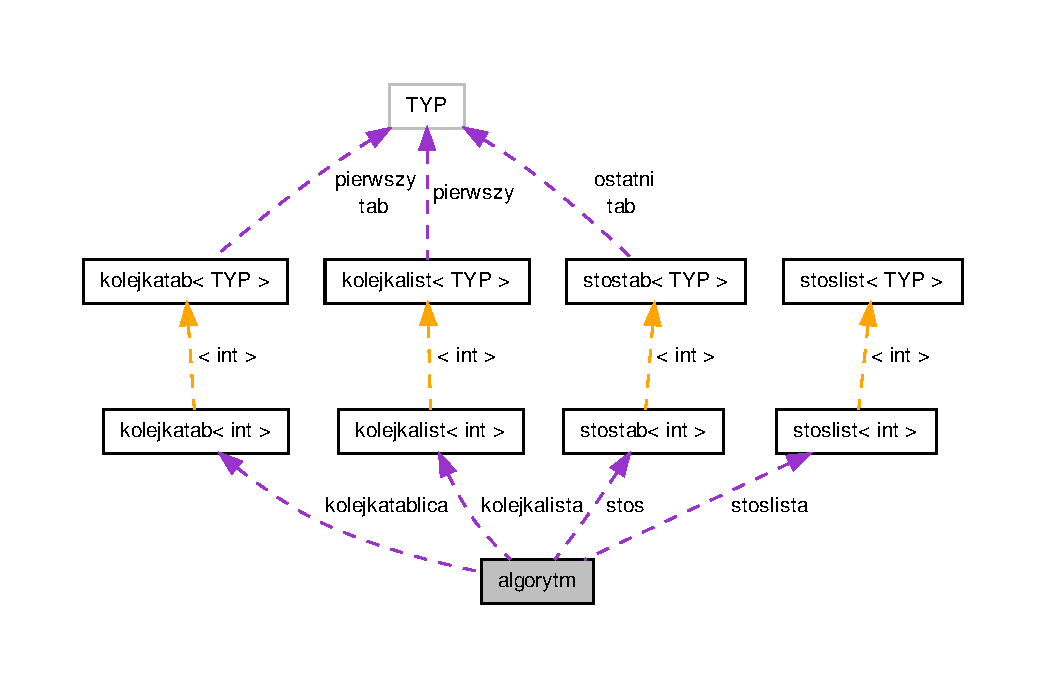
\includegraphics[width=350pt]{classalgorytm__coll__graph}
\end{center}
\end{figure}
\subsection*{Public Member Functions}
\begin{DoxyCompactItemize}
\item 
int $\ast$ \hyperlink{classalgorytm_aa2512ee12d0f4dd322b2ae38e0104728}{wczytaj\-\_\-dane} ()
\begin{DoxyCompactList}\small\item\em Metoda wczytujaca dane z pliku tesowego. \end{DoxyCompactList}\item 
void \hyperlink{classalgorytm_a6a50daab50bb9c7789103e480f8e2c0e}{wczytaj\-\_\-dane\-\_\-stostab} ()
\begin{DoxyCompactList}\small\item\em Metoda wczytujaca dane z pliku tekstowego do stosu implementowanego tablica. \end{DoxyCompactList}\item 
void \hyperlink{classalgorytm_af9ae4eedcaaa43665254cc40c3606f54}{wczytaj\-\_\-dane\-\_\-stoslista} ()
\begin{DoxyCompactList}\small\item\em Metoda wczytujaca dane z pliku tekstowego do stosu implementowanego lista. \end{DoxyCompactList}\item 
void \hyperlink{classalgorytm_a21851a809ea3ba6915d960c042fdba87}{wczytaj\-\_\-dane\-\_\-kolejkatab} ()
\begin{DoxyCompactList}\small\item\em Metoda wczytujaca dane z pliku tekstowego do kolejki implementowanej tablica. \end{DoxyCompactList}\item 
void \hyperlink{classalgorytm_a48d95d13b1f049c90a27cec0ef5e2c64}{wczytaj\-\_\-dane\-\_\-kolejkalist} ()
\begin{DoxyCompactList}\small\item\em Metoda wczytujaca dane z pliku tekstowego do kolejki implementowanej lista. \end{DoxyCompactList}\item 
void \hyperlink{classalgorytm_a5ace80a05bfc1305938d173753102ea2}{wlacz\-\_\-zegar} ()
\begin{DoxyCompactList}\small\item\em Metoda wlacz\-\_\-zegar. \end{DoxyCompactList}\item 
void \hyperlink{classalgorytm_a12c132e1a407f5dd38796f4d24308a6c}{wylacz\-\_\-zegar} ()
\begin{DoxyCompactList}\small\item\em Metoda wylacz\-\_\-zegar. \end{DoxyCompactList}\item 
int $\ast$ \hyperlink{classalgorytm_a78f39eb60ed01731efe1b69af93b0ab1}{wykonaj\-\_\-obliczenia} ()
\begin{DoxyCompactList}\small\item\em Metoda wykonaj obliczenia. \end{DoxyCompactList}\item 
int $\ast$ \hyperlink{classalgorytm_a218800ae392b95a6f257538940ee0c12}{wczytaj\-\_\-dane\-\_\-sprawdzajace} ()
\begin{DoxyCompactList}\small\item\em Metoda wczytujaca dane sprawdzajace z pliku tesowego. \end{DoxyCompactList}\item 
bool \hyperlink{classalgorytm_a238208b7d91fb5bf21c2262dfade6add}{sprawdz} ()
\begin{DoxyCompactList}\small\item\em Metoda Sprawdz. \end{DoxyCompactList}\item 
void \hyperlink{classalgorytm_ae0bcecdcf531d82d6f7fe07b669e8953}{zamien\-\_\-elementy} (int $\ast$tablica, int pierwszy, int drugi)
\begin{DoxyCompactList}\small\item\em Metoda zamien elementy. \end{DoxyCompactList}\item 
void \hyperlink{classalgorytm_acf5c24637c36aed90a4703c23d645e88}{odwroc\-\_\-tablice} (int $\ast$tablica)
\begin{DoxyCompactList}\small\item\em Metoda odwroc tablice. \end{DoxyCompactList}\item 
int $\ast$ \hyperlink{classalgorytm_abba1df6da457b63d6405de3191ecf8fc}{dodaj\-\_\-element} (int $\ast$tablica, int element)
\begin{DoxyCompactList}\small\item\em Metoda dodaj elementy. \end{DoxyCompactList}\item 
int $\ast$ \hyperlink{classalgorytm_a8ea259f4037d0ae2f8d3cffbafd9aa30}{dodaj\-\_\-elementy} (int $\ast$tab\-\_\-pierwsza, int $\ast$tab\-\_\-druga)
\begin{DoxyCompactList}\small\item\em Metoda dodaj elementy. \end{DoxyCompactList}\item 
int $\ast$ \hyperlink{classalgorytm_afc58371cc2a7d9355e03b7e0da204067}{operator=} (int $\ast$tab\-\_\-pierwsza)
\begin{DoxyCompactList}\small\item\em Przeciazenie operatora przypisania. \end{DoxyCompactList}\item 
int \hyperlink{classalgorytm_ac86c17db1372a20261b2eb66530d2775}{test} (\hyperlink{classdane}{dane} $\ast$Info)
\begin{DoxyCompactList}\small\item\em Metoda test. \end{DoxyCompactList}\item 
void \hyperlink{classalgorytm_ad5187dcb092d8c0ea27de1e2107f58fb}{test\-\_\-wczytania} (\hyperlink{classdane}{dane} $\ast$Info)
\begin{DoxyCompactList}\small\item\em Metoda test\-\_\-wczytania. \end{DoxyCompactList}\end{DoxyCompactItemize}
\subsection*{Public Attributes}
\begin{DoxyCompactItemize}
\item 
int \hyperlink{classalgorytm_a6f208bf8705cfe407a3b7dea8b1e871c}{powtorzenia}
\begin{DoxyCompactList}\small\item\em Pole powtorzenia. \end{DoxyCompactList}\item 
double \hyperlink{classalgorytm_a3d448d22ae50bd472f6daadd7bd24670}{czas\-\_\-nsec}
\begin{DoxyCompactList}\small\item\em Pole czas\-\_\-nsec. \end{DoxyCompactList}\item 
double \hyperlink{classalgorytm_a8e8e89b83e539607b01b5a33f8203d27}{czas\-\_\-sec}
\begin{DoxyCompactList}\small\item\em Pole czas\-\_\-sec;. \end{DoxyCompactList}\item 
int \hyperlink{classalgorytm_aa8284a41958410778215e08dc305f409}{elementy}
\begin{DoxyCompactList}\small\item\em Pole elementy. \end{DoxyCompactList}\item 
int $\ast$ \hyperlink{classalgorytm_a7bbde139599763bf8b36d21c6f314a1a}{tab\-\_\-danych}
\begin{DoxyCompactList}\small\item\em Wskaznik tab\-\_\-danych. \end{DoxyCompactList}\item 
int $\ast$ \hyperlink{classalgorytm_a02dd561c7411091f78e0d058bb1485df}{tab\-\_\-obliczone}
\begin{DoxyCompactList}\small\item\em Wskaznik tab\-\_\-obliczone. \end{DoxyCompactList}\item 
int $\ast$ \hyperlink{classalgorytm_a67ec91f63071c85dea86bed4b77d5239}{tab\-\_\-sprawdzajace}
\begin{DoxyCompactList}\small\item\em Wskaznik tab\-\_\-sprawdzajace. \end{DoxyCompactList}\item 
\hyperlink{classstostab}{stostab}$<$ int $>$ \hyperlink{classalgorytm_a1829772ca4b928e0df0e4af2fcf907ca}{stos}
\begin{DoxyCompactList}\small\item\em Obiekt stos klasy stostab. \end{DoxyCompactList}\item 
\hyperlink{classstoslist}{stoslist}$<$ int $>$ \hyperlink{classalgorytm_a334d547b11514cc290ea0395df44eda2}{stoslista}
\begin{DoxyCompactList}\small\item\em Obiekt stoslista klasy stoslist. \end{DoxyCompactList}\item 
\hyperlink{classkolejkalist}{kolejkalist}$<$ int $>$ \hyperlink{classalgorytm_a88d3998fb7af950b9bebe97898b7ab7a}{kolejkalista}
\begin{DoxyCompactList}\small\item\em Obiekt kolejkalista klasy kolejkalist. \end{DoxyCompactList}\item 
\hyperlink{classkolejkatab}{kolejkatab}$<$ int $>$ \hyperlink{classalgorytm_aefc3de70ca1ac1bf1ff0598229ddb915}{kolejkatablica}
\begin{DoxyCompactList}\small\item\em Obiekt kolejkatablica klasy kolejkatab. \end{DoxyCompactList}\end{DoxyCompactItemize}


\subsection{Detailed Description}
Klasa modeluje pojecie algorytmu w sklad ktorego wchodza pola odpowiadajace min. za ilosc wczytanych elementow, powtorzenia algorytmow. Wsrod metod klasy znajduja sie min. wczytanie danych, pobranie czasu, zamiana elementow tablicy itd. 

Definition at line 28 of file algorytm.\-h.



\subsection{Member Function Documentation}
\hypertarget{classalgorytm_abba1df6da457b63d6405de3191ecf8fc}{\index{algorytm@{algorytm}!dodaj\-\_\-element@{dodaj\-\_\-element}}
\index{dodaj\-\_\-element@{dodaj\-\_\-element}!algorytm@{algorytm}}
\subsubsection[{dodaj\-\_\-element}]{\setlength{\rightskip}{0pt plus 5cm}int $\ast$ algorytm\-::dodaj\-\_\-element (
\begin{DoxyParamCaption}
\item[{int $\ast$}]{tablica, }
\item[{int}]{element}
\end{DoxyParamCaption}
)}}\label{classalgorytm_abba1df6da457b63d6405de3191ecf8fc}
Metoda dodaj element dodaje do zadanej tablicy jeden element o zadanej wartosci na koniec tablicy przez co tablica zwieksza swoj rozmiar o 1. Metoda zwraca wskaznik na nowa tablice.


\begin{DoxyParams}[1]{Parameters}
\mbox{\tt in}  & {\em tablica} & -\/ wskaznik na tablice do ktorej zostanie dodany element. \\
\hline
\mbox{\tt in}  & {\em element} & -\/ zmienna typu int ktora zostanie dodana do podanej tablicy.\\
\hline
\end{DoxyParams}
\begin{DoxyReturn}{Returns}
Zwraca wskaznik do nowej tablicy z dodanym elementem. 
\end{DoxyReturn}


Definition at line 187 of file algorytm.\-cpp.

\hypertarget{classalgorytm_a8ea259f4037d0ae2f8d3cffbafd9aa30}{\index{algorytm@{algorytm}!dodaj\-\_\-elementy@{dodaj\-\_\-elementy}}
\index{dodaj\-\_\-elementy@{dodaj\-\_\-elementy}!algorytm@{algorytm}}
\subsubsection[{dodaj\-\_\-elementy}]{\setlength{\rightskip}{0pt plus 5cm}int $\ast$ algorytm\-::dodaj\-\_\-elementy (
\begin{DoxyParamCaption}
\item[{int $\ast$}]{tab\-\_\-pierwsza, }
\item[{int $\ast$}]{tab\-\_\-druga}
\end{DoxyParamCaption}
)}}\label{classalgorytm_a8ea259f4037d0ae2f8d3cffbafd9aa30}
Metoda dodaje ze soba dwie tablice tworzac jeden element. Jako argumenty metoda przyjmuje wskazniki na tablice ktore maja byc ze soba dodane. Zwracany jest wskaznik na nowo stworzona tablice zlozona z elementow obu tablic.


\begin{DoxyParams}[1]{Parameters}
\mbox{\tt in}  & {\em tab\-\_\-pierwsza} & -\/ tablica od ktorej bedzie rozpoczynala sie nowo utworzona tablica. \\
\hline
\mbox{\tt in}  & {\em tab\-\_\-druga} & -\/ tablica ktora zostanie dopisana jako druga do nowo utworzonej tablicy.\\
\hline
\end{DoxyParams}
\begin{DoxyReturn}{Returns}
Zwraca wskaznik na nowa tablice. 
\end{DoxyReturn}


Definition at line 197 of file algorytm.\-cpp.

\hypertarget{classalgorytm_acf5c24637c36aed90a4703c23d645e88}{\index{algorytm@{algorytm}!odwroc\-\_\-tablice@{odwroc\-\_\-tablice}}
\index{odwroc\-\_\-tablice@{odwroc\-\_\-tablice}!algorytm@{algorytm}}
\subsubsection[{odwroc\-\_\-tablice}]{\setlength{\rightskip}{0pt plus 5cm}void algorytm\-::odwroc\-\_\-tablice (
\begin{DoxyParamCaption}
\item[{int $\ast$}]{tablica}
\end{DoxyParamCaption}
)}}\label{classalgorytm_acf5c24637c36aed90a4703c23d645e88}
Metoda odwroc tablice wykonuje zamiane elementow tablicy w taki sposob iz pierwszy staje sie ostatni, a ostatni pierwszym. Jako argument przyjmuje wskaznik na tablice ktora chcemy odwrocic. Nie zwraca wartosci.


\begin{DoxyParams}[1]{Parameters}
\mbox{\tt in}  & {\em tablica} & -\/ wskaznik na tablice wartosci int. \\
\hline
\end{DoxyParams}


Definition at line 179 of file algorytm.\-cpp.

\hypertarget{classalgorytm_afc58371cc2a7d9355e03b7e0da204067}{\index{algorytm@{algorytm}!operator=@{operator=}}
\index{operator=@{operator=}!algorytm@{algorytm}}
\subsubsection[{operator=}]{\setlength{\rightskip}{0pt plus 5cm}int $\ast$ algorytm\-::operator= (
\begin{DoxyParamCaption}
\item[{int $\ast$}]{tab\-\_\-pierwsza}
\end{DoxyParamCaption}
)}}\label{classalgorytm_afc58371cc2a7d9355e03b7e0da204067}
Przeciazenie operatora przypisania pozwala na bezposrednie przypisanie dwoch tablic ze soba. Jako argument przyjmuje wskaznik na tablice ktora zostanie przypisana. Zwraca natomiast wskaznik na nowa tablice z przypisanymi elementami.


\begin{DoxyParams}[1]{Parameters}
\mbox{\tt in}  & {\em tab\-\_\-pierwsza} & -\/ wskaznik na tablice ktora bedzie przypisana do drugiej\\
\hline
\end{DoxyParams}
\begin{DoxyReturn}{Returns}
Zwraca wskaznik na ta tablice. 
\end{DoxyReturn}


Definition at line 209 of file algorytm.\-cpp.

\hypertarget{classalgorytm_a238208b7d91fb5bf21c2262dfade6add}{\index{algorytm@{algorytm}!sprawdz@{sprawdz}}
\index{sprawdz@{sprawdz}!algorytm@{algorytm}}
\subsubsection[{sprawdz}]{\setlength{\rightskip}{0pt plus 5cm}bool algorytm\-::sprawdz (
\begin{DoxyParamCaption}
{}
\end{DoxyParamCaption}
)}}\label{classalgorytm_a238208b7d91fb5bf21c2262dfade6add}
Metoda ta sprawdza poprawnosci wykonania operacji na tablicy danych poprzez porownanie kazdego elementu tab\-\_\-obliczone z odpowiadajacym jej elementem tab\-\_\-sprawdzjace. W przypadku poprawnego wykonania poprawnej operacji na tab\-\_\-danych i porownaniu z tab\-\_\-sprawdzajace metoda zwraca wartosc true gdy jakis z elementow jest inny od odpowiednika to zwracana jest wartosc false.

\begin{DoxyReturn}{Returns}
Zwraca wartosc logiczna true/false w zaleznosci od rezultatu. 
\end{DoxyReturn}


Definition at line 154 of file algorytm.\-cpp.

\hypertarget{classalgorytm_ac86c17db1372a20261b2eb66530d2775}{\index{algorytm@{algorytm}!test@{test}}
\index{test@{test}!algorytm@{algorytm}}
\subsubsection[{test}]{\setlength{\rightskip}{0pt plus 5cm}int algorytm\-::test (
\begin{DoxyParamCaption}
\item[{{\bf dane} $\ast$}]{Info}
\end{DoxyParamCaption}
)}}\label{classalgorytm_ac86c17db1372a20261b2eb66530d2775}
Metoda test jak nazwa wskazuje dokonuje poprawnosci dzialania zalozen programu. Sklada sie z odpowiedniej sekkwencji wywolania funkcji. Otwierane sa tu pliki testowe i sprawdzajace. Do obiektu Info sa wysylane odpowiednie informacje. Na koniec wywolywane sa metody klasy dane dokonujace zapisu danych statystycznych do pliku csv. Jako argument przyjmuje wskaznik do obiektu klasy dane. Zwraca wartosc logiczna 0 po wykonaniu testu


\begin{DoxyParams}[1]{Parameters}
\mbox{\tt in}  & {\em Info} & -\/ wskaznik na obiekt klasy dane do ktorego zapisane bd wyniki przeprowadzonego testu.\\
\hline
\end{DoxyParams}
\begin{DoxyReturn}{Returns}
Zwraca wartosc logiczna typu int po wykonaniu testu. 
\end{DoxyReturn}


Definition at line 218 of file algorytm.\-cpp.



Here is the call graph for this function\-:\nopagebreak
\begin{figure}[H]
\begin{center}
\leavevmode
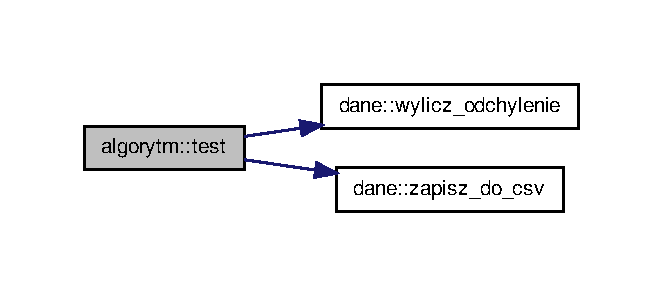
\includegraphics[width=318pt]{classalgorytm_ac86c17db1372a20261b2eb66530d2775_cgraph}
\end{center}
\end{figure}


\hypertarget{classalgorytm_ad5187dcb092d8c0ea27de1e2107f58fb}{\index{algorytm@{algorytm}!test\-\_\-wczytania@{test\-\_\-wczytania}}
\index{test\-\_\-wczytania@{test\-\_\-wczytania}!algorytm@{algorytm}}
\subsubsection[{test\-\_\-wczytania}]{\setlength{\rightskip}{0pt plus 5cm}void algorytm\-::test\-\_\-wczytania (
\begin{DoxyParamCaption}
\item[{{\bf dane} $\ast$}]{Info}
\end{DoxyParamCaption}
)}}\label{classalgorytm_ad5187dcb092d8c0ea27de1e2107f58fb}
Metoda test\-\_\-wczytania jest to metoda testujaca wczytywanie elementow z pliku oraz pomiar czasu tej operacji. Jako argument wejsciowy metoda przyjmuje wskaznik na obiekt typu dane. Nie zwracana jest zadna wartosc.


\begin{DoxyParams}[1]{Parameters}
\mbox{\tt in}  & {\em Info} & -\/ wskaznik na obiekt klasy dane \\
\hline
\end{DoxyParams}


Definition at line 236 of file algorytm.\-cpp.



Here is the call graph for this function\-:
\nopagebreak
\begin{figure}[H]
\begin{center}
\leavevmode
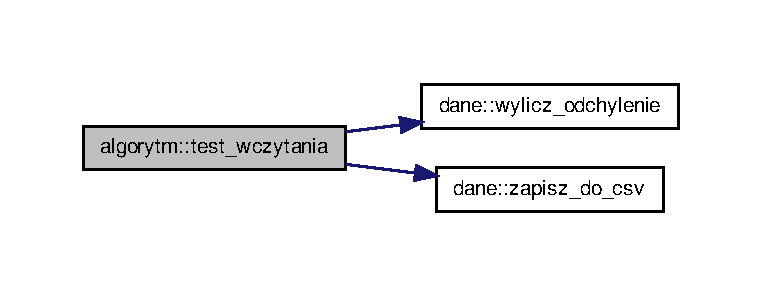
\includegraphics[width=350pt]{classalgorytm_ad5187dcb092d8c0ea27de1e2107f58fb_cgraph}
\end{center}
\end{figure}




Here is the caller graph for this function\-:
\nopagebreak
\begin{figure}[H]
\begin{center}
\leavevmode
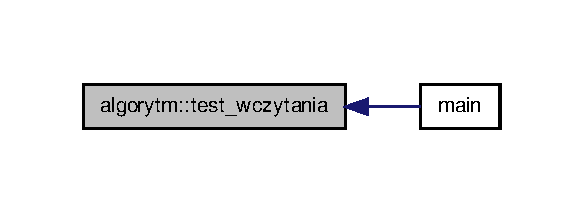
\includegraphics[width=280pt]{classalgorytm_ad5187dcb092d8c0ea27de1e2107f58fb_icgraph}
\end{center}
\end{figure}


\hypertarget{classalgorytm_aa2512ee12d0f4dd322b2ae38e0104728}{\index{algorytm@{algorytm}!wczytaj\-\_\-dane@{wczytaj\-\_\-dane}}
\index{wczytaj\-\_\-dane@{wczytaj\-\_\-dane}!algorytm@{algorytm}}
\subsubsection[{wczytaj\-\_\-dane}]{\setlength{\rightskip}{0pt plus 5cm}int $\ast$ algorytm\-::wczytaj\-\_\-dane (
\begin{DoxyParamCaption}
{}
\end{DoxyParamCaption}
)}}\label{classalgorytm_aa2512ee12d0f4dd322b2ae38e0104728}
Metoda ta wykonuje operacje wczytania pliku z danymi do tablicy tab\-\_\-danych zawierajacej dane int. rozmiar tablicy definiowany jest przez liczbe elementow okreslona przez pierwsza wartosc wczytana z pliku. W przypadku niepowodzenia operacji otwarcia pliku uzytkownik informowany jest o tym odpowiednim komunikatem. Metoda zwraca wskaznik na tablice z wczytanymi przez nia danymi.

\begin{DoxyReturn}{Returns}
Zwraca wskaznik na tab\-\_\-danych 
\end{DoxyReturn}


Definition at line 30 of file algorytm.\-cpp.

\hypertarget{classalgorytm_a48d95d13b1f049c90a27cec0ef5e2c64}{\index{algorytm@{algorytm}!wczytaj\-\_\-dane\-\_\-kolejkalist@{wczytaj\-\_\-dane\-\_\-kolejkalist}}
\index{wczytaj\-\_\-dane\-\_\-kolejkalist@{wczytaj\-\_\-dane\-\_\-kolejkalist}!algorytm@{algorytm}}
\subsubsection[{wczytaj\-\_\-dane\-\_\-kolejkalist}]{\setlength{\rightskip}{0pt plus 5cm}void algorytm\-::wczytaj\-\_\-dane\-\_\-kolejkalist (
\begin{DoxyParamCaption}
{}
\end{DoxyParamCaption}
)}}\label{classalgorytm_a48d95d13b1f049c90a27cec0ef5e2c64}
Metoda ta wykonuje operacje wczytywania pliku tekstowego z danymi do kolejki zaimplementowanej przy uzyciu szablonu listy z S\-T\-L wraz z wykorzystaniem jej metod. Metoda nie przyjmuje zadnych argumentow. Nie zwraca tez zadnych wartosci , w przypadku niepoprawnego otwarcia pliku uzytkownik jest informowany o tym fakcie odpowiednim komunikatem. 

Definition at line 100 of file algorytm.\-cpp.

\hypertarget{classalgorytm_a21851a809ea3ba6915d960c042fdba87}{\index{algorytm@{algorytm}!wczytaj\-\_\-dane\-\_\-kolejkatab@{wczytaj\-\_\-dane\-\_\-kolejkatab}}
\index{wczytaj\-\_\-dane\-\_\-kolejkatab@{wczytaj\-\_\-dane\-\_\-kolejkatab}!algorytm@{algorytm}}
\subsubsection[{wczytaj\-\_\-dane\-\_\-kolejkatab}]{\setlength{\rightskip}{0pt plus 5cm}void algorytm\-::wczytaj\-\_\-dane\-\_\-kolejkatab (
\begin{DoxyParamCaption}
{}
\end{DoxyParamCaption}
)}}\label{classalgorytm_a21851a809ea3ba6915d960c042fdba87}
Metoda ta wykonuje operacje wczytywania pliku tekstowego z danymi do kolejki zaimlementowanej przy użyciu tablicy alokowanej dynamicznie. Funkcja nie zwraca zadnej wartosci. W przypaku niepowodzenia operacji otwarcia pliku uzytkownik informowany jest o tym odpowiednim komunikatem. 

Definition at line 82 of file algorytm.\-cpp.

\hypertarget{classalgorytm_a218800ae392b95a6f257538940ee0c12}{\index{algorytm@{algorytm}!wczytaj\-\_\-dane\-\_\-sprawdzajace@{wczytaj\-\_\-dane\-\_\-sprawdzajace}}
\index{wczytaj\-\_\-dane\-\_\-sprawdzajace@{wczytaj\-\_\-dane\-\_\-sprawdzajace}!algorytm@{algorytm}}
\subsubsection[{wczytaj\-\_\-dane\-\_\-sprawdzajace}]{\setlength{\rightskip}{0pt plus 5cm}int $\ast$ algorytm\-::wczytaj\-\_\-dane\-\_\-sprawdzajace (
\begin{DoxyParamCaption}
{}
\end{DoxyParamCaption}
)}}\label{classalgorytm_a218800ae392b95a6f257538940ee0c12}
Metoda ta wykonuje operacje wczytania pliku z danymi do tablicy tab\-\_\-sprawdzajace zawierajacej dane int. rozmiar tablicy definiowany jest przez liczbe elementow okreslona przez pierwsza wartosc wczytana z pliku z danymi testowymi. W przypadku niepowodzenia operacji otwarcia pliku uzytkownik informowany jest o tym odpowiednim komunikatem. Metoda zwraca wskaznik na tablice z wczytanymi przez nia danymi sprawdzajacymi.

\begin{DoxyReturn}{Returns}
Zwraca wskaznik na tab\-\_\-sprawdzajace. 
\end{DoxyReturn}


Definition at line 137 of file algorytm.\-cpp.

\hypertarget{classalgorytm_af9ae4eedcaaa43665254cc40c3606f54}{\index{algorytm@{algorytm}!wczytaj\-\_\-dane\-\_\-stoslista@{wczytaj\-\_\-dane\-\_\-stoslista}}
\index{wczytaj\-\_\-dane\-\_\-stoslista@{wczytaj\-\_\-dane\-\_\-stoslista}!algorytm@{algorytm}}
\subsubsection[{wczytaj\-\_\-dane\-\_\-stoslista}]{\setlength{\rightskip}{0pt plus 5cm}void algorytm\-::wczytaj\-\_\-dane\-\_\-stoslista (
\begin{DoxyParamCaption}
{}
\end{DoxyParamCaption}
)}}\label{classalgorytm_af9ae4eedcaaa43665254cc40c3606f54}
Metoda ta wykonuje operacje wczytywania pliku tekstowego z danymi do stosu zaimlementowanego przy użyciu listy z S\-T\-L. Funkcja nie zwraca zadnej wartosci. W przypaku niepowodzenia operacji otwarcia pliku uzytkownik informowany jest o tym odpowiednim komunikatem. 

Definition at line 65 of file algorytm.\-cpp.

\hypertarget{classalgorytm_a6a50daab50bb9c7789103e480f8e2c0e}{\index{algorytm@{algorytm}!wczytaj\-\_\-dane\-\_\-stostab@{wczytaj\-\_\-dane\-\_\-stostab}}
\index{wczytaj\-\_\-dane\-\_\-stostab@{wczytaj\-\_\-dane\-\_\-stostab}!algorytm@{algorytm}}
\subsubsection[{wczytaj\-\_\-dane\-\_\-stostab}]{\setlength{\rightskip}{0pt plus 5cm}void algorytm\-::wczytaj\-\_\-dane\-\_\-stostab (
\begin{DoxyParamCaption}
{}
\end{DoxyParamCaption}
)}}\label{classalgorytm_a6a50daab50bb9c7789103e480f8e2c0e}
Metoda ta wykonuje operacje wczytywania pliku tekstowego z danymi do stosu zaimlementowanego przy użyciu tablicy alokowanej dynamicznie. Funkcja nie zwraca zadnej wartosci. W przypaku niepowodzenia operacji otwarcia pliku uzytkownik informowany jest o tym odpowiednim komunikatem. 

Definition at line 48 of file algorytm.\-cpp.

\hypertarget{classalgorytm_a5ace80a05bfc1305938d173753102ea2}{\index{algorytm@{algorytm}!wlacz\-\_\-zegar@{wlacz\-\_\-zegar}}
\index{wlacz\-\_\-zegar@{wlacz\-\_\-zegar}!algorytm@{algorytm}}
\subsubsection[{wlacz\-\_\-zegar}]{\setlength{\rightskip}{0pt plus 5cm}void algorytm\-::wlacz\-\_\-zegar (
\begin{DoxyParamCaption}
{}
\end{DoxyParamCaption}
)}}\label{classalgorytm_a5ace80a05bfc1305938d173753102ea2}
Metoda sluzy do wlaczenia zegara i wykorzystania w obliczeniach czasu w jakim wykonany zostal algorytm oraz kazde jego powtorzenie. Nie zwraca wartosci. 

Definition at line 117 of file algorytm.\-cpp.

\hypertarget{classalgorytm_a78f39eb60ed01731efe1b69af93b0ab1}{\index{algorytm@{algorytm}!wykonaj\-\_\-obliczenia@{wykonaj\-\_\-obliczenia}}
\index{wykonaj\-\_\-obliczenia@{wykonaj\-\_\-obliczenia}!algorytm@{algorytm}}
\subsubsection[{wykonaj\-\_\-obliczenia}]{\setlength{\rightskip}{0pt plus 5cm}int $\ast$ algorytm\-::wykonaj\-\_\-obliczenia (
\begin{DoxyParamCaption}
{}
\end{DoxyParamCaption}
)}}\label{classalgorytm_a78f39eb60ed01731efe1b69af93b0ab1}
Metoda sluzy do wykonywania obliczen na tablicy znajdujacej sie w polu klasy Algorytm. Funkcja zwraca wskaznik na tablice z danymi po wykonaniu operacji na nich.

\begin{DoxyReturn}{Returns}
Wskaznik na tab\-\_\-obliczone. 
\end{DoxyReturn}


Definition at line 129 of file algorytm.\-cpp.

\hypertarget{classalgorytm_a12c132e1a407f5dd38796f4d24308a6c}{\index{algorytm@{algorytm}!wylacz\-\_\-zegar@{wylacz\-\_\-zegar}}
\index{wylacz\-\_\-zegar@{wylacz\-\_\-zegar}!algorytm@{algorytm}}
\subsubsection[{wylacz\-\_\-zegar}]{\setlength{\rightskip}{0pt plus 5cm}void algorytm\-::wylacz\-\_\-zegar (
\begin{DoxyParamCaption}
{}
\end{DoxyParamCaption}
)}}\label{classalgorytm_a12c132e1a407f5dd38796f4d24308a6c}
Metoda sluzy do wylaczenia zegara o wykonaniu sie danego algorytmu. Metoda nie zwraca zadnych wartosci. 

Definition at line 123 of file algorytm.\-cpp.

\hypertarget{classalgorytm_ae0bcecdcf531d82d6f7fe07b669e8953}{\index{algorytm@{algorytm}!zamien\-\_\-elementy@{zamien\-\_\-elementy}}
\index{zamien\-\_\-elementy@{zamien\-\_\-elementy}!algorytm@{algorytm}}
\subsubsection[{zamien\-\_\-elementy}]{\setlength{\rightskip}{0pt plus 5cm}void algorytm\-::zamien\-\_\-elementy (
\begin{DoxyParamCaption}
\item[{int $\ast$}]{tablica, }
\item[{int}]{pierwszy, }
\item[{int}]{drugi}
\end{DoxyParamCaption}
)}}\label{classalgorytm_ae0bcecdcf531d82d6f7fe07b669e8953}
Metoda zamien elementy dokonuje zamiany elementow o zadanych parametrach. Jako parametry metoda przyjmuje wskaznik na tablice na ktorej chcemy wykonac operacje oraz dwa kolejne argumenty typu int, ktore podaja numer elementu ktore maja byc ze soba zamienione. Zadna wartosc nie jest zwracana.


\begin{DoxyParams}[1]{Parameters}
\mbox{\tt in}  & {\em tablica} & -\/ wskaznik na tablice, w ktorej chcemy zamienic elementy. \\
\hline
\mbox{\tt in}  & {\em pierwszy} & -\/ pierwszy z elementow tablicy ktore chcemy zamienic. \\
\hline
\mbox{\tt in}  & {\em drugi} & -\/ drug z elementow tablicy ktore chcemy ze soba zamienic. \\
\hline
\end{DoxyParams}


Definition at line 173 of file algorytm.\-cpp.



\subsection{Member Data Documentation}
\hypertarget{classalgorytm_a3d448d22ae50bd472f6daadd7bd24670}{\index{algorytm@{algorytm}!czas\-\_\-nsec@{czas\-\_\-nsec}}
\index{czas\-\_\-nsec@{czas\-\_\-nsec}!algorytm@{algorytm}}
\subsubsection[{czas\-\_\-nsec}]{\setlength{\rightskip}{0pt plus 5cm}double algorytm\-::czas\-\_\-nsec}}\label{classalgorytm_a3d448d22ae50bd472f6daadd7bd24670}
Pole odpowiada za przechowywanie nano czesci czasu wykonania operacji. 

Definition at line 43 of file algorytm.\-h.

\hypertarget{classalgorytm_a8e8e89b83e539607b01b5a33f8203d27}{\index{algorytm@{algorytm}!czas\-\_\-sec@{czas\-\_\-sec}}
\index{czas\-\_\-sec@{czas\-\_\-sec}!algorytm@{algorytm}}
\subsubsection[{czas\-\_\-sec}]{\setlength{\rightskip}{0pt plus 5cm}double algorytm\-::czas\-\_\-sec}}\label{classalgorytm_a8e8e89b83e539607b01b5a33f8203d27}
Pole czas\-\_\-sec odpowiada za przechowywanie liczby sekund wykonania danego powtorzenia. 

Definition at line 50 of file algorytm.\-h.

\hypertarget{classalgorytm_aa8284a41958410778215e08dc305f409}{\index{algorytm@{algorytm}!elementy@{elementy}}
\index{elementy@{elementy}!algorytm@{algorytm}}
\subsubsection[{elementy}]{\setlength{\rightskip}{0pt plus 5cm}int algorytm\-::elementy}}\label{classalgorytm_aa8284a41958410778215e08dc305f409}
Pole to odpowiedzialne jest za przechowywanie informacji mowiacej o ilosci elementow jaka pozostanie wczytana do programu z pliku tekstowego. 

Definition at line 58 of file algorytm.\-h.

\hypertarget{classalgorytm_a88d3998fb7af950b9bebe97898b7ab7a}{\index{algorytm@{algorytm}!kolejkalista@{kolejkalista}}
\index{kolejkalista@{kolejkalista}!algorytm@{algorytm}}
\subsubsection[{kolejkalista}]{\setlength{\rightskip}{0pt plus 5cm}{\bf kolejkalist}$<$int$>$ algorytm\-::kolejkalista}}\label{classalgorytm_a88d3998fb7af950b9bebe97898b7ab7a}
Obiekt kolejkalista jest szablonem klasy kolejkalist oznaczajacym kolejke zaimplementowana przy uzyciu szablonu listy z biblioteki S\-T\-L. 

Definition at line 108 of file algorytm.\-h.

\hypertarget{classalgorytm_aefc3de70ca1ac1bf1ff0598229ddb915}{\index{algorytm@{algorytm}!kolejkatablica@{kolejkatablica}}
\index{kolejkatablica@{kolejkatablica}!algorytm@{algorytm}}
\subsubsection[{kolejkatablica}]{\setlength{\rightskip}{0pt plus 5cm}{\bf kolejkatab}$<$int$>$ algorytm\-::kolejkatablica}}\label{classalgorytm_aefc3de70ca1ac1bf1ff0598229ddb915}
Obiekt kolejkatablica jest kolejka zaimplementowana przy uzyciu szablonu klasy kolejkatab. Klasa ta wykorzystuje implementacje przy uzyciu tablicy alokowanej dynamicznie. 

Definition at line 117 of file algorytm.\-h.

\hypertarget{classalgorytm_a6f208bf8705cfe407a3b7dea8b1e871c}{\index{algorytm@{algorytm}!powtorzenia@{powtorzenia}}
\index{powtorzenia@{powtorzenia}!algorytm@{algorytm}}
\subsubsection[{powtorzenia}]{\setlength{\rightskip}{0pt plus 5cm}int algorytm\-::powtorzenia}}\label{classalgorytm_a6f208bf8705cfe407a3b7dea8b1e871c}
Pole to odpowiedzialne jest za przechowywanie informacji mowiacej o ilosci powtorzen algorytmu. 

Definition at line 36 of file algorytm.\-h.

\hypertarget{classalgorytm_a1829772ca4b928e0df0e4af2fcf907ca}{\index{algorytm@{algorytm}!stos@{stos}}
\index{stos@{stos}!algorytm@{algorytm}}
\subsubsection[{stos}]{\setlength{\rightskip}{0pt plus 5cm}{\bf stostab}$<$int$>$ algorytm\-::stos}}\label{classalgorytm_a1829772ca4b928e0df0e4af2fcf907ca}
Obiekt ten jest szablonem obiektu klasy stostab oznaczajacy stos zaimplementowany na bazie tablicy alokowanej dynamicznie 

Definition at line 92 of file algorytm.\-h.

\hypertarget{classalgorytm_a334d547b11514cc290ea0395df44eda2}{\index{algorytm@{algorytm}!stoslista@{stoslista}}
\index{stoslista@{stoslista}!algorytm@{algorytm}}
\subsubsection[{stoslista}]{\setlength{\rightskip}{0pt plus 5cm}{\bf stoslist}$<$int$>$ algorytm\-::stoslista}}\label{classalgorytm_a334d547b11514cc290ea0395df44eda2}
Obiekt ten jest szablonem obiektu klasy stoslist oznaczajacym stos zaimplementowany na bazie szablonu listy z S\-T\-L. 

Definition at line 100 of file algorytm.\-h.

\hypertarget{classalgorytm_a7bbde139599763bf8b36d21c6f314a1a}{\index{algorytm@{algorytm}!tab\-\_\-danych@{tab\-\_\-danych}}
\index{tab\-\_\-danych@{tab\-\_\-danych}!algorytm@{algorytm}}
\subsubsection[{tab\-\_\-danych}]{\setlength{\rightskip}{0pt plus 5cm}int$\ast$ algorytm\-::tab\-\_\-danych}}\label{classalgorytm_a7bbde139599763bf8b36d21c6f314a1a}
Pole to odpowiedzialne jest za przechowywanie wskaznika do alokowanej dynamicznie tablicy danych zawierajacej elementy wczytane z pliku testowego. 

Definition at line 67 of file algorytm.\-h.

\hypertarget{classalgorytm_a02dd561c7411091f78e0d058bb1485df}{\index{algorytm@{algorytm}!tab\-\_\-obliczone@{tab\-\_\-obliczone}}
\index{tab\-\_\-obliczone@{tab\-\_\-obliczone}!algorytm@{algorytm}}
\subsubsection[{tab\-\_\-obliczone}]{\setlength{\rightskip}{0pt plus 5cm}int$\ast$ algorytm\-::tab\-\_\-obliczone}}\label{classalgorytm_a02dd561c7411091f78e0d058bb1485df}
Pole to odpowiedzialne jest za przechowywanie wskaznika do alokowanej dynamicznie tablicy danych zawierajacej wartosci elementow z tablicy danych przez okreslona wartosc. 

Definition at line 76 of file algorytm.\-h.

\hypertarget{classalgorytm_a67ec91f63071c85dea86bed4b77d5239}{\index{algorytm@{algorytm}!tab\-\_\-sprawdzajace@{tab\-\_\-sprawdzajace}}
\index{tab\-\_\-sprawdzajace@{tab\-\_\-sprawdzajace}!algorytm@{algorytm}}
\subsubsection[{tab\-\_\-sprawdzajace}]{\setlength{\rightskip}{0pt plus 5cm}int$\ast$ algorytm\-::tab\-\_\-sprawdzajace}}\label{classalgorytm_a67ec91f63071c85dea86bed4b77d5239}
Pole to odpowiedzialne jest za przechowywanie wskaznika do alokowanej dynamicznie tablicy danych zawierajacej wartosci elementow z tablicy danych przez okreslona wartosc. 

Definition at line 85 of file algorytm.\-h.



The documentation for this class was generated from the following files\-:\begin{DoxyCompactItemize}
\item 
\hyperlink{algorytm_8h}{algorytm.\-h}\item 
\hyperlink{algorytm_8cpp}{algorytm.\-cpp}\end{DoxyCompactItemize}

\hypertarget{classdane}{\section{dane Class Reference}
\label{classdane}\index{dane@{dane}}
}


Modeluje pojecie dane.  




{\ttfamily \#include $<$dane.\-h$>$}

\subsection*{Public Member Functions}
\begin{DoxyCompactItemize}
\item 
\hyperlink{classdane_aa74e7fb3542aa856cf6e36d5cd9a4db9}{dane} (int \hyperlink{classdane_a77efb8d7494e984418802f6e7cc32d20}{powtorzenia})
\begin{DoxyCompactList}\small\item\em Konstruktor parametryczny. \end{DoxyCompactList}\item 
void \hyperlink{classdane_a365e299198fea0ee26fe080de6b0d12e}{wylicz\-\_\-odchylenie} ()
\begin{DoxyCompactList}\small\item\em Metoda wyliczajaca odchylenie standardowe. \end{DoxyCompactList}\item 
void \hyperlink{classdane_a8427efc3e40d63911205b297aecb4ca9}{zapisz\-\_\-do\-\_\-csv} ()
\begin{DoxyCompactList}\small\item\em Metoda zapisujaca dane do pliku csv. \end{DoxyCompactList}\end{DoxyCompactItemize}
\subsection*{Public Attributes}
\begin{DoxyCompactItemize}
\item 
int \hyperlink{classdane_a77efb8d7494e984418802f6e7cc32d20}{powtorzenia}
\begin{DoxyCompactList}\small\item\em Pole powtorzenia. \end{DoxyCompactList}\item 
double \hyperlink{classdane_af0dccb6c88a06aaf08441cc01d6bff27}{czas\-\_\-operacji}
\begin{DoxyCompactList}\small\item\em Pole czas\-\_\-operacji. \end{DoxyCompactList}\item 
double \hyperlink{classdane_adf1201c327225fc441f65b6d3b0d17e9}{odchylenie}
\begin{DoxyCompactList}\small\item\em Pole odchylenie. \end{DoxyCompactList}\item 
double $\ast$ \hyperlink{classdane_a722f3af9d9a100995ebaba0fc63e6e25}{tab\-\_\-czasow}
\begin{DoxyCompactList}\small\item\em Pole $\ast$tab\-\_\-czasow. \end{DoxyCompactList}\end{DoxyCompactItemize}


\subsection{Detailed Description}
Klasa modeluje pojecie dane. W tej klasie znajduja sie informacje dotyczace podsumowania pracy algorytmu. Polami tej klasy sa zmienne odpowiadajace za min. ilosc powtorzen algorytmu. Metody tej klasy wyliczaja odchylenie standardowe oraz zapisuja dane podsumowujace w pliku csv. 

Definition at line 26 of file dane.\-h.



\subsection{Constructor \& Destructor Documentation}
\hypertarget{classdane_aa74e7fb3542aa856cf6e36d5cd9a4db9}{\index{dane@{dane}!dane@{dane}}
\index{dane@{dane}!dane@{dane}}
\subsubsection[{dane}]{\setlength{\rightskip}{0pt plus 5cm}dane\-::dane (
\begin{DoxyParamCaption}
\item[{int}]{powtorzenia}
\end{DoxyParamCaption}
)}}\label{classdane_aa74e7fb3542aa856cf6e36d5cd9a4db9}
Konstruktor jako parametr przyjmuje wartosc powtorzen, aby zaalokowac pamiec potrzebna do przechowywania czasu kazdego powtorzenia algorytmu. 

Definition at line 20 of file dane.\-cpp.



\subsection{Member Function Documentation}
\hypertarget{classdane_a365e299198fea0ee26fe080de6b0d12e}{\index{dane@{dane}!wylicz\-\_\-odchylenie@{wylicz\-\_\-odchylenie}}
\index{wylicz\-\_\-odchylenie@{wylicz\-\_\-odchylenie}!dane@{dane}}
\subsubsection[{wylicz\-\_\-odchylenie}]{\setlength{\rightskip}{0pt plus 5cm}void dane\-::wylicz\-\_\-odchylenie (
\begin{DoxyParamCaption}
{}
\end{DoxyParamCaption}
)}}\label{classdane_a365e299198fea0ee26fe080de6b0d12e}
Metoda ta wylicza wartosc odchylenia standardowego zestawu czasow zawartych w tablicy czasow tab\-\_\-czasow. Metoda nie przyjmuje parametrow, ani nie zwraca zadnej wartosci. 

Definition at line 23 of file dane.\-cpp.



Here is the caller graph for this function\-:
\nopagebreak
\begin{figure}[H]
\begin{center}
\leavevmode
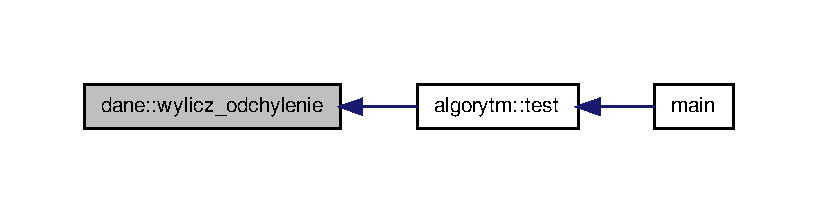
\includegraphics[width=350pt]{classdane_a365e299198fea0ee26fe080de6b0d12e_icgraph}
\end{center}
\end{figure}


\hypertarget{classdane_a8427efc3e40d63911205b297aecb4ca9}{\index{dane@{dane}!zapisz\-\_\-do\-\_\-csv@{zapisz\-\_\-do\-\_\-csv}}
\index{zapisz\-\_\-do\-\_\-csv@{zapisz\-\_\-do\-\_\-csv}!dane@{dane}}
\subsubsection[{zapisz\-\_\-do\-\_\-csv}]{\setlength{\rightskip}{0pt plus 5cm}void dane\-::zapisz\-\_\-do\-\_\-csv (
\begin{DoxyParamCaption}
{}
\end{DoxyParamCaption}
)}}\label{classdane_a8427efc3e40d63911205b297aecb4ca9}
Metoda ta zapisuje informacje dotyczace wykonania sie algorytmu w pliku formatu csv. W tej metodzie tworzony jest odpowiedni obiekt klasy fstream do ktorego zapisywane sa informacje odnosnie ilosci powtorzen, czasu operacji, czasu powtorzen oraz odchylenie standardowe czasow. 

Definition at line 38 of file dane.\-cpp.



Here is the caller graph for this function\-:
\nopagebreak
\begin{figure}[H]
\begin{center}
\leavevmode
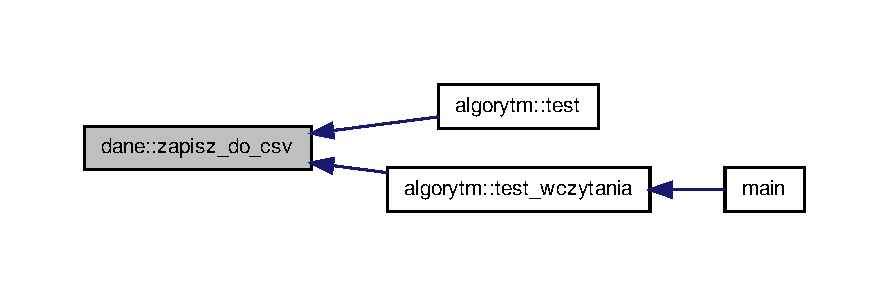
\includegraphics[width=350pt]{classdane_a8427efc3e40d63911205b297aecb4ca9_icgraph}
\end{center}
\end{figure}




\subsection{Member Data Documentation}
\hypertarget{classdane_af0dccb6c88a06aaf08441cc01d6bff27}{\index{dane@{dane}!czas\-\_\-operacji@{czas\-\_\-operacji}}
\index{czas\-\_\-operacji@{czas\-\_\-operacji}!dane@{dane}}
\subsubsection[{czas\-\_\-operacji}]{\setlength{\rightskip}{0pt plus 5cm}double dane\-::czas\-\_\-operacji}}\label{classdane_af0dccb6c88a06aaf08441cc01d6bff27}
Pole to odpowiedzialne jest za przechowywanie informacji mowiacej w jakim czasie wykonano wszystkie powtorzenia algorytmu. Zmienna jest typu double. 

Definition at line 43 of file dane.\-h.

\hypertarget{classdane_adf1201c327225fc441f65b6d3b0d17e9}{\index{dane@{dane}!odchylenie@{odchylenie}}
\index{odchylenie@{odchylenie}!dane@{dane}}
\subsubsection[{odchylenie}]{\setlength{\rightskip}{0pt plus 5cm}double dane\-::odchylenie}}\label{classdane_adf1201c327225fc441f65b6d3b0d17e9}
Pole to odpowiedzialne jest za przechowywanie informacji mowiacej ile wynosi odchylenie standardowe z czasow wykonania algorytmu. Zmienna jest typu double. 

Definition at line 51 of file dane.\-h.

\hypertarget{classdane_a77efb8d7494e984418802f6e7cc32d20}{\index{dane@{dane}!powtorzenia@{powtorzenia}}
\index{powtorzenia@{powtorzenia}!dane@{dane}}
\subsubsection[{powtorzenia}]{\setlength{\rightskip}{0pt plus 5cm}int dane\-::powtorzenia}}\label{classdane_a77efb8d7494e984418802f6e7cc32d20}
Pole to odpowiedzialne jest za przechowywanie informacji mowiacej o ilosci powtorzen algorytmu. Zmienna jest typu int. 

Definition at line 35 of file dane.\-h.

\hypertarget{classdane_a722f3af9d9a100995ebaba0fc63e6e25}{\index{dane@{dane}!tab\-\_\-czasow@{tab\-\_\-czasow}}
\index{tab\-\_\-czasow@{tab\-\_\-czasow}!dane@{dane}}
\subsubsection[{tab\-\_\-czasow}]{\setlength{\rightskip}{0pt plus 5cm}double$\ast$ dane\-::tab\-\_\-czasow}}\label{classdane_a722f3af9d9a100995ebaba0fc63e6e25}
Pole to odpowiedzialne jest za przechowywanie czasow kazdego powtorzenia. Jest ono wskaznikiem na te tablice, ktora jest alokowana w sposob dynamiczny. Ilosc elementow okreslona jest przez ilosc powtorzen algorytmu. 

Definition at line 60 of file dane.\-h.



The documentation for this class was generated from the following files\-:\begin{DoxyCompactItemize}
\item 
\hyperlink{dane_8h}{dane.\-h}\item 
\hyperlink{dane_8cpp}{dane.\-cpp}\end{DoxyCompactItemize}

\hypertarget{classkolejkalist}{\section{kolejkalist$<$ T\-Y\-P $>$ Class Template Reference}
\label{classkolejkalist}\index{kolejkalist$<$ T\-Y\-P $>$@{kolejkalist$<$ T\-Y\-P $>$}}
}


Definicja klasy kolejkalist.  




{\ttfamily \#include $<$kolejka.\-h$>$}



Inheritance diagram for kolejkalist$<$ T\-Y\-P $>$\-:\nopagebreak
\begin{figure}[H]
\begin{center}
\leavevmode
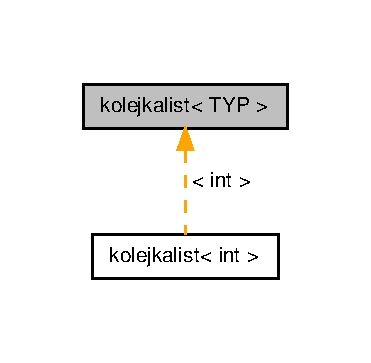
\includegraphics[width=178pt]{classkolejkalist__inherit__graph}
\end{center}
\end{figure}


Collaboration diagram for kolejkalist$<$ T\-Y\-P $>$\-:\nopagebreak
\begin{figure}[H]
\begin{center}
\leavevmode
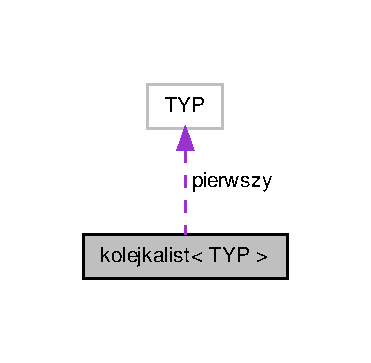
\includegraphics[width=178pt]{classkolejkalist__coll__graph}
\end{center}
\end{figure}
\subsection*{Public Member Functions}
\begin{DoxyCompactItemize}
\item 
\hyperlink{classkolejkalist_a90513e8c4cc0551dbe4e7d6bc2bbc1ee}{kolejkalist} ()
\begin{DoxyCompactList}\small\item\em Konstruktor klasy kolejkalist. \end{DoxyCompactList}\item 
int \hyperlink{classkolejkalist_a9ebc4dc0f552161532501b6e7d6483ae}{size} ()
\begin{DoxyCompactList}\small\item\em Metoda size. \end{DoxyCompactList}\item 
bool \hyperlink{classkolejkalist_a5cfccf441eb0fab70fb7f03d1f5edc23}{empty} ()
\begin{DoxyCompactList}\small\item\em Metoda empty. \end{DoxyCompactList}\item 
void \hyperlink{classkolejkalist_adda98f8350ae43dbef3367e2f0d90735}{enqueue} (T\-Y\-P element)
\begin{DoxyCompactList}\small\item\em Metoda enqueue. \end{DoxyCompactList}\item 
void \hyperlink{classkolejkalist_a06f0c76eb9579d6dd76ff354f2c16b1c}{dequeue} ()
\begin{DoxyCompactList}\small\item\em Metoda dequeue. \end{DoxyCompactList}\end{DoxyCompactItemize}
\subsection*{Public Attributes}
\begin{DoxyCompactItemize}
\item 
list$<$ T\-Y\-P $>$ \hyperlink{classkolejkalist_a303c82cb7875fd2779679a0e937900c0}{lista}
\begin{DoxyCompactList}\small\item\em Pole lista. \end{DoxyCompactList}\item 
T\-Y\-P \hyperlink{classkolejkalist_a62f458a961a2179f5c8977bae73fe42b}{pierwszy}
\begin{DoxyCompactList}\small\item\em Pole pierwszy. \end{DoxyCompactList}\end{DoxyCompactItemize}


\subsection{Detailed Description}
\subsubsection*{template$<$typename T\-Y\-P$>$class kolejkalist$<$ T\-Y\-P $>$}

Szablon klasy kolejkalist jest implementacja listy na bazie listy z kontenera S\-T\-L. W sklad szablonu wchodzi szablon listy oraz pole klasy pierwszy typu T\-Y\-P przechowujacy pierwszy element po wykonaniu operacji pobrania elemnetu. 

Definition at line 29 of file kolejka.\-h.



\subsection{Constructor \& Destructor Documentation}
\hypertarget{classkolejkalist_a90513e8c4cc0551dbe4e7d6bc2bbc1ee}{\index{kolejkalist@{kolejkalist}!kolejkalist@{kolejkalist}}
\index{kolejkalist@{kolejkalist}!kolejkalist@{kolejkalist}}
\subsubsection[{kolejkalist}]{\setlength{\rightskip}{0pt plus 5cm}template$<$typename T\-Y\-P$>$ {\bf kolejkalist}$<$ T\-Y\-P $>$\-::{\bf kolejkalist} (
\begin{DoxyParamCaption}
{}
\end{DoxyParamCaption}
)\hspace{0.3cm}{\ttfamily [inline]}}}\label{classkolejkalist_a90513e8c4cc0551dbe4e7d6bc2bbc1ee}
W konstruktorze klasy inicjalizowana jest wartosc zmiennej pierwszy. 

Definition at line 54 of file kolejka.\-h.



\subsection{Member Function Documentation}
\hypertarget{classkolejkalist_a06f0c76eb9579d6dd76ff354f2c16b1c}{\index{kolejkalist@{kolejkalist}!dequeue@{dequeue}}
\index{dequeue@{dequeue}!kolejkalist@{kolejkalist}}
\subsubsection[{dequeue}]{\setlength{\rightskip}{0pt plus 5cm}template$<$typename T\-Y\-P$>$ void {\bf kolejkalist}$<$ T\-Y\-P $>$\-::dequeue (
\begin{DoxyParamCaption}
{}
\end{DoxyParamCaption}
)\hspace{0.3cm}{\ttfamily [inline]}}}\label{classkolejkalist_a06f0c76eb9579d6dd76ff354f2c16b1c}
Metoda ta zabiera pierwszy element znajdujacy sie w kolejce. Nie przyjmuje zadnych argumentow oraz nie zwraca zadnych wartosci. W przypadku braku elementow w kolejce uzytkownik jest informowany o tym fakcie odpowiednim komunikatem. 

Definition at line 108 of file kolejka.\-h.

\hypertarget{classkolejkalist_a5cfccf441eb0fab70fb7f03d1f5edc23}{\index{kolejkalist@{kolejkalist}!empty@{empty}}
\index{empty@{empty}!kolejkalist@{kolejkalist}}
\subsubsection[{empty}]{\setlength{\rightskip}{0pt plus 5cm}template$<$typename T\-Y\-P$>$ bool {\bf kolejkalist}$<$ T\-Y\-P $>$\-::empty (
\begin{DoxyParamCaption}
{}
\end{DoxyParamCaption}
)\hspace{0.3cm}{\ttfamily [inline]}}}\label{classkolejkalist_a5cfccf441eb0fab70fb7f03d1f5edc23}
Metoda ta sprawdza czy w kolejce znajduja sie jakiekolwiek elementy. Sprawdza ona warunek czy rozmiar kolejki zwracany w metodzie size jest rowny 0. Jeśli tak to zwraca wartosc logiczna true jesli nie to zwraca wartosc false. Metoda nie pobiera zadnych argumentow.

\begin{DoxyReturn}{Returns}
Zwraca wartosc logiczna w zaleznosci od wyniku operacji porownania 
\end{DoxyReturn}


Definition at line 80 of file kolejka.\-h.

\hypertarget{classkolejkalist_adda98f8350ae43dbef3367e2f0d90735}{\index{kolejkalist@{kolejkalist}!enqueue@{enqueue}}
\index{enqueue@{enqueue}!kolejkalist@{kolejkalist}}
\subsubsection[{enqueue}]{\setlength{\rightskip}{0pt plus 5cm}template$<$typename T\-Y\-P$>$ void {\bf kolejkalist}$<$ T\-Y\-P $>$\-::enqueue (
\begin{DoxyParamCaption}
\item[{T\-Y\-P}]{element}
\end{DoxyParamCaption}
)\hspace{0.3cm}{\ttfamily [inline]}}}\label{classkolejkalist_adda98f8350ae43dbef3367e2f0d90735}
Metoda enqueue dodaje element na koniec kolejki. Wykorzystuje do tego metode z szablonu listy push\-\_\-back ktora dodaje element na koniec listy. Metoda pobiera argument element typu T\-Y\-P. Nie zwraca zadnych wartosci.


\begin{DoxyParams}[1]{Parameters}
\mbox{\tt in}  & {\em element} & -\/ element ktory ma byc dolozony na koniec kolejki \\
\hline
\end{DoxyParams}


Definition at line 97 of file kolejka.\-h.

\hypertarget{classkolejkalist_a9ebc4dc0f552161532501b6e7d6483ae}{\index{kolejkalist@{kolejkalist}!size@{size}}
\index{size@{size}!kolejkalist@{kolejkalist}}
\subsubsection[{size}]{\setlength{\rightskip}{0pt plus 5cm}template$<$typename T\-Y\-P$>$ int {\bf kolejkalist}$<$ T\-Y\-P $>$\-::size (
\begin{DoxyParamCaption}
{}
\end{DoxyParamCaption}
)\hspace{0.3cm}{\ttfamily [inline]}}}\label{classkolejkalist_a9ebc4dc0f552161532501b6e7d6483ae}
Metoda size podaje ilosc elementow znajdujacych sie w kolejce. Zwraca wynik funkci size z szablonu listy. Wartosc ta jest typu calkowitego.

\begin{DoxyReturn}{Returns}
Zwraca ilosc elementow w kolejce 
\end{DoxyReturn}


Definition at line 66 of file kolejka.\-h.



\subsection{Member Data Documentation}
\hypertarget{classkolejkalist_a303c82cb7875fd2779679a0e937900c0}{\index{kolejkalist@{kolejkalist}!lista@{lista}}
\index{lista@{lista}!kolejkalist@{kolejkalist}}
\subsubsection[{lista}]{\setlength{\rightskip}{0pt plus 5cm}template$<$typename T\-Y\-P$>$ list$<$T\-Y\-P$>$ {\bf kolejkalist}$<$ T\-Y\-P $>$\-::lista}}\label{classkolejkalist_a303c82cb7875fd2779679a0e937900c0}
Pole lista jest szablonem listy zmiennych typu T\-Y\-P. W niej przechowywane sa elementy ktore dodawane sa do kolejki. 

Definition at line 38 of file kolejka.\-h.

\hypertarget{classkolejkalist_a62f458a961a2179f5c8977bae73fe42b}{\index{kolejkalist@{kolejkalist}!pierwszy@{pierwszy}}
\index{pierwszy@{pierwszy}!kolejkalist@{kolejkalist}}
\subsubsection[{pierwszy}]{\setlength{\rightskip}{0pt plus 5cm}template$<$typename T\-Y\-P$>$ T\-Y\-P {\bf kolejkalist}$<$ T\-Y\-P $>$\-::pierwszy}}\label{classkolejkalist_a62f458a961a2179f5c8977bae73fe42b}
Pole pierwszy jest zmienna typu takiego jaki zostanie podany przez uzytkownika w momencie tworzenia obiektu. Przechowywana w nim jest wartosc elementu ktory jako ostatni zostal pobrany z kolejki. 

Definition at line 47 of file kolejka.\-h.



The documentation for this class was generated from the following file\-:\begin{DoxyCompactItemize}
\item 
\hyperlink{kolejka_8h}{kolejka.\-h}\end{DoxyCompactItemize}

\hypertarget{classkolejkatab}{\section{kolejkatab$<$ T\-Y\-P $>$ Class Template Reference}
\label{classkolejkatab}\index{kolejkatab$<$ T\-Y\-P $>$@{kolejkatab$<$ T\-Y\-P $>$}}
}


Szablon klasy kolejkatab.  




{\ttfamily \#include $<$kolejka.\-h$>$}



Inheritance diagram for kolejkatab$<$ T\-Y\-P $>$\-:\nopagebreak
\begin{figure}[H]
\begin{center}
\leavevmode
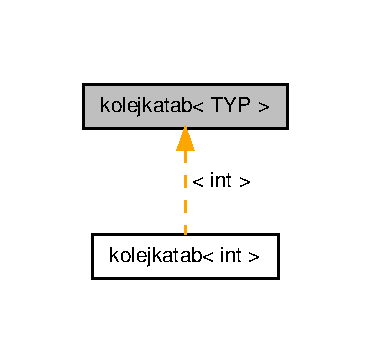
\includegraphics[width=178pt]{classkolejkatab__inherit__graph}
\end{center}
\end{figure}


Collaboration diagram for kolejkatab$<$ T\-Y\-P $>$\-:\nopagebreak
\begin{figure}[H]
\begin{center}
\leavevmode
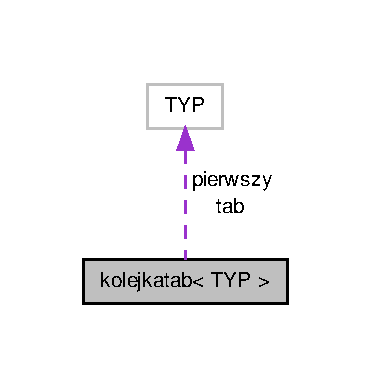
\includegraphics[width=178pt]{classkolejkatab__coll__graph}
\end{center}
\end{figure}
\subsection*{Public Member Functions}
\begin{DoxyCompactItemize}
\item 
\hyperlink{classkolejkatab_ae8f978affe7d275f38b432ba89eddce7}{kolejkatab} ()
\begin{DoxyCompactList}\small\item\em Konstruktor klasy kolejkatab. \end{DoxyCompactList}\item 
T\-Y\-P $\ast$ \hyperlink{classkolejkatab_a19cfea1a6282ec8a3e7f7d903bad4ec0}{tworz} (int N)
\begin{DoxyCompactList}\small\item\em Metoda tworz. \end{DoxyCompactList}\item 
bool \hyperlink{classkolejkatab_a3a15f6d2fe43f387e60d63f11b68d0a5}{empty} ()
\begin{DoxyCompactList}\small\item\em Metoda empty. \end{DoxyCompactList}\item 
int \hyperlink{classkolejkatab_ab2bd484f25e38850871321cf8c695271}{size} ()
\begin{DoxyCompactList}\small\item\em Metoda size. \end{DoxyCompactList}\item 
void \hyperlink{classkolejkatab_a6ba37d3ed63eb91be0ec150dc0646c50}{enqueue\-\_\-dod} (T\-Y\-P element)
\begin{DoxyCompactList}\small\item\em Metoda enqueue\-\_\-dod. \end{DoxyCompactList}\item 
void \hyperlink{classkolejkatab_a1f4b14e081aef543ff4e08e2060042cb}{enqueue\-\_\-pom} (T\-Y\-P element)
\begin{DoxyCompactList}\small\item\em Metoda enqueue\-\_\-pom. \end{DoxyCompactList}\item 
void \hyperlink{classkolejkatab_ae15cc5e580f16def922ce447f38dbab5}{dequeue} ()
\begin{DoxyCompactList}\small\item\em Metoda dequeue. \end{DoxyCompactList}\item 
void \hyperlink{classkolejkatab_ab7b360e73b75756d96a1aa6a102e7318}{clear} ()
\begin{DoxyCompactList}\small\item\em Metoda clear. \end{DoxyCompactList}\end{DoxyCompactItemize}
\subsection*{Public Attributes}
\begin{DoxyCompactItemize}
\item 
int \hyperlink{classkolejkatab_a77ad076380322b9698305c608aab6637}{rozmiar}
\begin{DoxyCompactList}\small\item\em Pole rozmiar. \end{DoxyCompactList}\item 
T\-Y\-P $\ast$ \hyperlink{classkolejkatab_a91ec1706d1e10ce7f781a5102c4b59b8}{tab}
\begin{DoxyCompactList}\small\item\em Pole wskaznika na tablice. \end{DoxyCompactList}\item 
unsigned int \hyperlink{classkolejkatab_a161d4a2c4e17bd942ca79ae3a421ff34}{ilosc}
\begin{DoxyCompactList}\small\item\em Pole ilosc. \end{DoxyCompactList}\item 
T\-Y\-P \hyperlink{classkolejkatab_a9eac0eb1ac26bedc608938e7865b6352}{pierwszy}
\begin{DoxyCompactList}\small\item\em Pole pierwszy. \end{DoxyCompactList}\end{DoxyCompactItemize}


\subsection{Detailed Description}
\subsubsection*{template$<$typename T\-Y\-P$>$class kolejkatab$<$ T\-Y\-P $>$}

Szablon klasy kolejkatab jest implementacja kolejki w oparciu o tablice alokowana dynamicznie. W szablonie znajduja sie wszystkie niezbedne metody do poprawnego funkcjonowania obiektow jako kolejek. 

Definition at line 128 of file kolejka.\-h.



\subsection{Constructor \& Destructor Documentation}
\hypertarget{classkolejkatab_ae8f978affe7d275f38b432ba89eddce7}{\index{kolejkatab@{kolejkatab}!kolejkatab@{kolejkatab}}
\index{kolejkatab@{kolejkatab}!kolejkatab@{kolejkatab}}
\subsubsection[{kolejkatab}]{\setlength{\rightskip}{0pt plus 5cm}template$<$typename T\-Y\-P$>$ {\bf kolejkatab}$<$ T\-Y\-P $>$\-::{\bf kolejkatab} (
\begin{DoxyParamCaption}
{}
\end{DoxyParamCaption}
)\hspace{0.3cm}{\ttfamily [inline]}}}\label{classkolejkatab_ae8f978affe7d275f38b432ba89eddce7}
Konstruktor klasy kolejkatab. W nim przypisywana jest wartosc poczatkowa polom ilosc oraz rozmiar. 

Definition at line 167 of file kolejka.\-h.



\subsection{Member Function Documentation}
\hypertarget{classkolejkatab_ab7b360e73b75756d96a1aa6a102e7318}{\index{kolejkatab@{kolejkatab}!clear@{clear}}
\index{clear@{clear}!kolejkatab@{kolejkatab}}
\subsubsection[{clear}]{\setlength{\rightskip}{0pt plus 5cm}template$<$typename T\-Y\-P$>$ void {\bf kolejkatab}$<$ T\-Y\-P $>$\-::clear (
\begin{DoxyParamCaption}
{}
\end{DoxyParamCaption}
)\hspace{0.3cm}{\ttfamily [inline]}}}\label{classkolejkatab_ab7b360e73b75756d96a1aa6a102e7318}
Metoda wykonujaca operacje sciagniecia wszytskich elementow z kolejki. Zapobiega przed nadpisywaniem wartosci. 

Definition at line 329 of file kolejka.\-h.

\hypertarget{classkolejkatab_ae15cc5e580f16def922ce447f38dbab5}{\index{kolejkatab@{kolejkatab}!dequeue@{dequeue}}
\index{dequeue@{dequeue}!kolejkatab@{kolejkatab}}
\subsubsection[{dequeue}]{\setlength{\rightskip}{0pt plus 5cm}template$<$typename T\-Y\-P$>$ void {\bf kolejkatab}$<$ T\-Y\-P $>$\-::dequeue (
\begin{DoxyParamCaption}
{}
\end{DoxyParamCaption}
)\hspace{0.3cm}{\ttfamily [inline]}}}\label{classkolejkatab_ae15cc5e580f16def922ce447f38dbab5}
Metoda usuwajaca pierwszy element z kolejki. W przypadku gdy w kolejce nie ma elementow operacja usuniecia elementu nie zostanie wykonana. Uzytkownik jest o tym fakcie informowany odpowiednim komunikatem. Gdy kolejka wypelniona jest w co najmniej w 1/4 to rozmiar zaalokowanej tablicy zmniejszany jest o polowe. Metoda nie zwraca zadnych wartosci. Wartosc usunietego elementu przechowywana jest w polu pierwszy dopoki nie zostanie wykonana kolejna operacja usuniecia elementu z kolejki. 

Definition at line 292 of file kolejka.\-h.

\hypertarget{classkolejkatab_a3a15f6d2fe43f387e60d63f11b68d0a5}{\index{kolejkatab@{kolejkatab}!empty@{empty}}
\index{empty@{empty}!kolejkatab@{kolejkatab}}
\subsubsection[{empty}]{\setlength{\rightskip}{0pt plus 5cm}template$<$typename T\-Y\-P$>$ bool {\bf kolejkatab}$<$ T\-Y\-P $>$\-::empty (
\begin{DoxyParamCaption}
{}
\end{DoxyParamCaption}
)\hspace{0.3cm}{\ttfamily [inline]}}}\label{classkolejkatab_a3a15f6d2fe43f387e60d63f11b68d0a5}
Metoda empty sluzy do sprawdzenia czy w kolejce znajduja sie jakies elementy. Jesli wartosc zwracana przez metoda size jest inna od 0 wtedy funkcja zwraca wartosc false. W przypadku prawdziwosci warunku zwracana jest wartosc true.

\begin{DoxyReturn}{Returns}
Zwraca wartosc logiczna w zaleznosci od warunku petli 
\end{DoxyReturn}


Definition at line 198 of file kolejka.\-h.

\hypertarget{classkolejkatab_a6ba37d3ed63eb91be0ec150dc0646c50}{\index{kolejkatab@{kolejkatab}!enqueue\-\_\-dod@{enqueue\-\_\-dod}}
\index{enqueue\-\_\-dod@{enqueue\-\_\-dod}!kolejkatab@{kolejkatab}}
\subsubsection[{enqueue\-\_\-dod}]{\setlength{\rightskip}{0pt plus 5cm}template$<$typename T\-Y\-P$>$ void {\bf kolejkatab}$<$ T\-Y\-P $>$\-::enqueue\-\_\-dod (
\begin{DoxyParamCaption}
\item[{T\-Y\-P}]{element}
\end{DoxyParamCaption}
)\hspace{0.3cm}{\ttfamily [inline]}}}\label{classkolejkatab_a6ba37d3ed63eb91be0ec150dc0646c50}
Metoda enqueue\-\_\-dod dokonuje dodania elementu na koniec kolejki. W przypadku kiedy tablica do ktorej wprowadzane sa wartosci jest zapelniona to jej rozmiar zwiekszany jest o 1. Jako argument metoda przyjmuje wartosc elementu typu T\-Y\-P. Nie zwraca zadnych wartosci.


\begin{DoxyParams}[1]{Parameters}
\mbox{\tt in}  & {\em element} & -\/ zmienna typu T\-Y\-P dodawana na koniec kolejki \\
\hline
\end{DoxyParams}


Definition at line 228 of file kolejka.\-h.

\hypertarget{classkolejkatab_a1f4b14e081aef543ff4e08e2060042cb}{\index{kolejkatab@{kolejkatab}!enqueue\-\_\-pom@{enqueue\-\_\-pom}}
\index{enqueue\-\_\-pom@{enqueue\-\_\-pom}!kolejkatab@{kolejkatab}}
\subsubsection[{enqueue\-\_\-pom}]{\setlength{\rightskip}{0pt plus 5cm}template$<$typename T\-Y\-P$>$ void {\bf kolejkatab}$<$ T\-Y\-P $>$\-::enqueue\-\_\-pom (
\begin{DoxyParamCaption}
\item[{T\-Y\-P}]{element}
\end{DoxyParamCaption}
)\hspace{0.3cm}{\ttfamily [inline]}}}\label{classkolejkatab_a1f4b14e081aef543ff4e08e2060042cb}
Metoda enqueue\-\_\-dod dokonuje dodania elementu na koniec kolejki. W przypadku kiedy tablica do ktorej wprowadzane sa wartosci jest zapelniona to jej rozmiar zwiekszany dwukrotnie. Jako argument metoda przyjmuje wartosc elementu typu T\-Y\-P. Nie zwraca zadnych wartosci.


\begin{DoxyParams}[1]{Parameters}
\mbox{\tt in}  & {\em element} & -\/ zmienna typu T\-Y\-P dodawana na koniec kolejki \\
\hline
\end{DoxyParams}


Definition at line 259 of file kolejka.\-h.

\hypertarget{classkolejkatab_ab2bd484f25e38850871321cf8c695271}{\index{kolejkatab@{kolejkatab}!size@{size}}
\index{size@{size}!kolejkatab@{kolejkatab}}
\subsubsection[{size}]{\setlength{\rightskip}{0pt plus 5cm}template$<$typename T\-Y\-P$>$ int {\bf kolejkatab}$<$ T\-Y\-P $>$\-::size (
\begin{DoxyParamCaption}
{}
\end{DoxyParamCaption}
)\hspace{0.3cm}{\ttfamily [inline]}}}\label{classkolejkatab_ab2bd484f25e38850871321cf8c695271}
Metoda size sluzy do podania ilosci elementow w kolejce. Zwraca aktualna wartosc zmiennej ilosc. Zwracana wartosc jest typu int.

\begin{DoxyReturn}{Returns}
Zwraca wartosc zmiennej ilosc. 
\end{DoxyReturn}


Definition at line 213 of file kolejka.\-h.

\hypertarget{classkolejkatab_a19cfea1a6282ec8a3e7f7d903bad4ec0}{\index{kolejkatab@{kolejkatab}!tworz@{tworz}}
\index{tworz@{tworz}!kolejkatab@{kolejkatab}}
\subsubsection[{tworz}]{\setlength{\rightskip}{0pt plus 5cm}template$<$typename T\-Y\-P$>$ T\-Y\-P$\ast$ {\bf kolejkatab}$<$ T\-Y\-P $>$\-::tworz (
\begin{DoxyParamCaption}
\item[{int}]{N}
\end{DoxyParamCaption}
)\hspace{0.3cm}{\ttfamily [inline]}}}\label{classkolejkatab_a19cfea1a6282ec8a3e7f7d903bad4ec0}
Metoda tworz tworzy tablice dynamiczna o zadanym rozmiarze. Jako argument przyjmuje zmienna N typu int. Metoda zwraca wskaznik na tablice typow T\-Y\-P.


\begin{DoxyParams}[1]{Parameters}
\mbox{\tt in}  & {\em N} & -\/ wartosc rozmiaru zadeklarowanej tablicy\\
\hline
\end{DoxyParams}
\begin{DoxyReturn}{Returns}
Wskaznik na tablice typow T\-Y\-P 
\end{DoxyReturn}


Definition at line 182 of file kolejka.\-h.



\subsection{Member Data Documentation}
\hypertarget{classkolejkatab_a161d4a2c4e17bd942ca79ae3a421ff34}{\index{kolejkatab@{kolejkatab}!ilosc@{ilosc}}
\index{ilosc@{ilosc}!kolejkatab@{kolejkatab}}
\subsubsection[{ilosc}]{\setlength{\rightskip}{0pt plus 5cm}template$<$typename T\-Y\-P$>$ unsigned int {\bf kolejkatab}$<$ T\-Y\-P $>$\-::ilosc}}\label{classkolejkatab_a161d4a2c4e17bd942ca79ae3a421ff34}
Pole ilosc odpowiada za przechowywanie informacji ile elementow znajduje sie w kolejce. Sluzy do sprawdzenia wypelnienia tablicy. 

Definition at line 152 of file kolejka.\-h.

\hypertarget{classkolejkatab_a9eac0eb1ac26bedc608938e7865b6352}{\index{kolejkatab@{kolejkatab}!pierwszy@{pierwszy}}
\index{pierwszy@{pierwszy}!kolejkatab@{kolejkatab}}
\subsubsection[{pierwszy}]{\setlength{\rightskip}{0pt plus 5cm}template$<$typename T\-Y\-P$>$ T\-Y\-P {\bf kolejkatab}$<$ T\-Y\-P $>$\-::pierwszy}}\label{classkolejkatab_a9eac0eb1ac26bedc608938e7865b6352}
Pole pierwszy przechowuje wartosc pierwszego elementu znajdujacego sie w kolejce. 

Definition at line 160 of file kolejka.\-h.

\hypertarget{classkolejkatab_a77ad076380322b9698305c608aab6637}{\index{kolejkatab@{kolejkatab}!rozmiar@{rozmiar}}
\index{rozmiar@{rozmiar}!kolejkatab@{kolejkatab}}
\subsubsection[{rozmiar}]{\setlength{\rightskip}{0pt plus 5cm}template$<$typename T\-Y\-P$>$ int {\bf kolejkatab}$<$ T\-Y\-P $>$\-::rozmiar}}\label{classkolejkatab_a77ad076380322b9698305c608aab6637}
Rozmiar jest zmienna typu int ktora przechowuje rozmiar zaalokowanej dynamicznie tablicy w ktorej znajduje sie kolejka. 

Definition at line 136 of file kolejka.\-h.

\hypertarget{classkolejkatab_a91ec1706d1e10ce7f781a5102c4b59b8}{\index{kolejkatab@{kolejkatab}!tab@{tab}}
\index{tab@{tab}!kolejkatab@{kolejkatab}}
\subsubsection[{tab}]{\setlength{\rightskip}{0pt plus 5cm}template$<$typename T\-Y\-P$>$ T\-Y\-P$\ast$ {\bf kolejkatab}$<$ T\-Y\-P $>$\-::tab}}\label{classkolejkatab_a91ec1706d1e10ce7f781a5102c4b59b8}
Pole to jest wskaznikiem na tablice tab ktora bedzie przechowywala elementy znajdujace sie w kolejce. Zainicjowanie tablicy dokonuje sie w w metodzie tworz po podaniu rozmiaru tablicy. 

Definition at line 144 of file kolejka.\-h.



The documentation for this class was generated from the following file\-:\begin{DoxyCompactItemize}
\item 
\hyperlink{kolejka_8h}{kolejka.\-h}\end{DoxyCompactItemize}

\hypertarget{classstoslist}{\section{stoslist$<$ T\-Y\-P $>$ Class Template Reference}
\label{classstoslist}\index{stoslist$<$ T\-Y\-P $>$@{stoslist$<$ T\-Y\-P $>$}}
}


Definicja szablonu stoslist.  




{\ttfamily \#include $<$stos.\-h$>$}



Inheritance diagram for stoslist$<$ T\-Y\-P $>$\-:\nopagebreak
\begin{figure}[H]
\begin{center}
\leavevmode
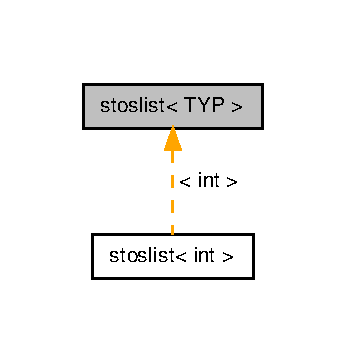
\includegraphics[width=166pt]{classstoslist__inherit__graph}
\end{center}
\end{figure}
\subsection*{Public Member Functions}
\begin{DoxyCompactItemize}
\item 
int \hyperlink{classstoslist_a5bf76e0da8be5a74aca69cde32768572}{size} ()
\begin{DoxyCompactList}\small\item\em Metoda size. \end{DoxyCompactList}\item 
bool \hyperlink{classstoslist_adfcff6fccf977218b512def56b285f4f}{empty} ()
\begin{DoxyCompactList}\small\item\em Metoda empty. \end{DoxyCompactList}\item 
void \hyperlink{classstoslist_af307aa8a238c1ae5b223bbb903210086}{push} (T\-Y\-P element)
\begin{DoxyCompactList}\small\item\em Metoda push. \end{DoxyCompactList}\item 
void \hyperlink{classstoslist_aca316220c9241b4fcff1e3bfce72eee1}{pop} ()
\begin{DoxyCompactList}\small\item\em Metoda pop. \end{DoxyCompactList}\end{DoxyCompactItemize}
\subsection*{Public Attributes}
\begin{DoxyCompactItemize}
\item 
list$<$ T\-Y\-P $>$ \hyperlink{classstoslist_ae1f96afc2ccdf5769f0b9242deedd12c}{lista}
\begin{DoxyCompactList}\small\item\em Pole lista. \end{DoxyCompactList}\item 
T\-Y\-P \hyperlink{classstoslist_a3e7308b3ec7f4fef6a6675e4471f5d74}{ostatni}
\begin{DoxyCompactList}\small\item\em Pole ostatni. \end{DoxyCompactList}\end{DoxyCompactItemize}


\subsection{Detailed Description}
\subsubsection*{template$<$typename T\-Y\-P$>$class stoslist$<$ T\-Y\-P $>$}

Szablon stoslist jest implementacja stosu przy uzyciu szablonu listy dostepnego w S\-T\-L list. W sklad szablonu wchodzi uzyty jako pole klasy szablon listy dzialajacy dla roznych typow danych oraz pole ostatni ktore przechowuje ostatni element znajdujacy sie na stosie. 

Definition at line 27 of file stos.\-h.



\subsection{Member Function Documentation}
\hypertarget{classstoslist_adfcff6fccf977218b512def56b285f4f}{\index{stoslist@{stoslist}!empty@{empty}}
\index{empty@{empty}!stoslist@{stoslist}}
\subsubsection[{empty}]{\setlength{\rightskip}{0pt plus 5cm}template$<$typename T\-Y\-P$>$ bool {\bf stoslist}$<$ T\-Y\-P $>$\-::empty (
\begin{DoxyParamCaption}
{}
\end{DoxyParamCaption}
)\hspace{0.3cm}{\ttfamily [inline]}}}\label{classstoslist_adfcff6fccf977218b512def56b285f4f}
Metoda empty sprawdza czy na stosie znajduja sie elementy. Jesli wynik wartosci zwracanej przez metode size jest inny od 0 to funkcja zwraca wartosc logiczna false. W przypadku gdy metoda size zwraca wartosc 0 to zwracana jest wartosc logiczna true.

\begin{DoxyReturn}{Returns}
Zwraca w zaleznosci od wyniku true badz false 
\end{DoxyReturn}


Definition at line 66 of file stos.\-h.

\hypertarget{classstoslist_aca316220c9241b4fcff1e3bfce72eee1}{\index{stoslist@{stoslist}!pop@{pop}}
\index{pop@{pop}!stoslist@{stoslist}}
\subsubsection[{pop}]{\setlength{\rightskip}{0pt plus 5cm}template$<$typename T\-Y\-P$>$ void {\bf stoslist}$<$ T\-Y\-P $>$\-::pop (
\begin{DoxyParamCaption}
{}
\end{DoxyParamCaption}
)\hspace{0.3cm}{\ttfamily [inline]}}}\label{classstoslist_aca316220c9241b4fcff1e3bfce72eee1}
Metoda pop odpowiada za zabranie elementu ze stosu (z konca listy). W tej metodzie wykorzystywana jest metoda pop\-\_\-back ktora usuwa ostatni element z listy. Przed wykonaniem usuniecia elementu z listy do pola ostatni zapisywana jest wartosc ostatniego elementu znajdujacego sie w liscie. Przed wykonaniem jakiejkolwiek operacji sprawdzana jest liczba elementow na stosie. W przypadku gdy na stosie nie nie ma zadnego elementu to nie mozna wykonac operacji pobrania elementu ze stosu. W przypadku wywolania funkcji pop bez elementu na stosie. Uzytkownik informowany jest odpowiednim komunikatem o braku elementow na stosie. Metoda nie przyjmuje ani też nie zwraca zadnych elementow. 

Definition at line 104 of file stos.\-h.

\hypertarget{classstoslist_af307aa8a238c1ae5b223bbb903210086}{\index{stoslist@{stoslist}!push@{push}}
\index{push@{push}!stoslist@{stoslist}}
\subsubsection[{push}]{\setlength{\rightskip}{0pt plus 5cm}template$<$typename T\-Y\-P$>$ void {\bf stoslist}$<$ T\-Y\-P $>$\-::push (
\begin{DoxyParamCaption}
\item[{T\-Y\-P}]{element}
\end{DoxyParamCaption}
)\hspace{0.3cm}{\ttfamily [inline]}}}\label{classstoslist_af307aa8a238c1ae5b223bbb903210086}
Metoda push odpowiada za dodanie elementu do stosu (na koniec listy). Metoda bazuje na metodzie obiektu lista push\-\_\-back, ktora dodaje element na koniec listy. Jako parametr wejsciowy metoda przyjmuje zmienna typu T\-Y\-P. Metoda nie zwraca zadnej wartosci.


\begin{DoxyParams}[1]{Parameters}
\mbox{\tt in}  & {\em element} & -\/ element ktory ma zostac dodany do struktury stosu \\
\hline
\end{DoxyParams}


Definition at line 83 of file stos.\-h.

\hypertarget{classstoslist_a5bf76e0da8be5a74aca69cde32768572}{\index{stoslist@{stoslist}!size@{size}}
\index{size@{size}!stoslist@{stoslist}}
\subsubsection[{size}]{\setlength{\rightskip}{0pt plus 5cm}template$<$typename T\-Y\-P$>$ int {\bf stoslist}$<$ T\-Y\-P $>$\-::size (
\begin{DoxyParamCaption}
{}
\end{DoxyParamCaption}
)\hspace{0.3cm}{\ttfamily [inline]}}}\label{classstoslist_a5bf76e0da8be5a74aca69cde32768572}
Metoda size podaje ilosc elementow znajdujacych sie na stosie. Zwraca ona wynik metody z obiektu list.

\begin{DoxyReturn}{Returns}
Zwraca wartosc typu int wyniku metody lista.\-size() 
\end{DoxyReturn}


Definition at line 52 of file stos.\-h.



\subsection{Member Data Documentation}
\hypertarget{classstoslist_ae1f96afc2ccdf5769f0b9242deedd12c}{\index{stoslist@{stoslist}!lista@{lista}}
\index{lista@{lista}!stoslist@{stoslist}}
\subsubsection[{lista}]{\setlength{\rightskip}{0pt plus 5cm}template$<$typename T\-Y\-P$>$ list$<$T\-Y\-P$>$ {\bf stoslist}$<$ T\-Y\-P $>$\-::lista}}\label{classstoslist_ae1f96afc2ccdf5769f0b9242deedd12c}
Lista jest to miejsce przechowywania danych umieszczanych na stosie. Jest to obiekt typu list na bazie szablonu i dziala dla roznych typu danych. 

Definition at line 36 of file stos.\-h.

\hypertarget{classstoslist_a3e7308b3ec7f4fef6a6675e4471f5d74}{\index{stoslist@{stoslist}!ostatni@{ostatni}}
\index{ostatni@{ostatni}!stoslist@{stoslist}}
\subsubsection[{ostatni}]{\setlength{\rightskip}{0pt plus 5cm}template$<$typename T\-Y\-P$>$ T\-Y\-P {\bf stoslist}$<$ T\-Y\-P $>$\-::ostatni}}\label{classstoslist_a3e7308b3ec7f4fef6a6675e4471f5d74}
Pole to odpowiada za przechowanie wartosci ostatniego elementu (pierwszy z gory) znajdujacego sie na stosie. 

Definition at line 43 of file stos.\-h.



The documentation for this class was generated from the following file\-:\begin{DoxyCompactItemize}
\item 
\hyperlink{stos_8h}{stos.\-h}\end{DoxyCompactItemize}

\hypertarget{classstostab}{\section{stostab$<$ T\-Y\-P $>$ Class Template Reference}
\label{classstostab}\index{stostab$<$ T\-Y\-P $>$@{stostab$<$ T\-Y\-P $>$}}
}


Definicja szablonu stostab.  




{\ttfamily \#include $<$stos.\-h$>$}



Inheritance diagram for stostab$<$ T\-Y\-P $>$\-:\nopagebreak
\begin{figure}[H]
\begin{center}
\leavevmode
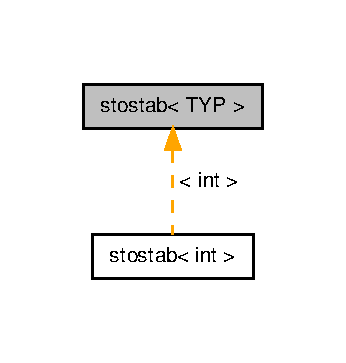
\includegraphics[width=166pt]{classstostab__inherit__graph}
\end{center}
\end{figure}


Collaboration diagram for stostab$<$ T\-Y\-P $>$\-:
\nopagebreak
\begin{figure}[H]
\begin{center}
\leavevmode
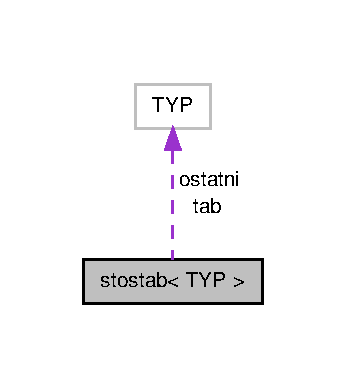
\includegraphics[width=166pt]{classstostab__coll__graph}
\end{center}
\end{figure}
\subsection*{Public Member Functions}
\begin{DoxyCompactItemize}
\item 
\hyperlink{classstostab_a496c66f7d32ff4ceb5fd833582c75e79}{stostab} ()
\begin{DoxyCompactList}\small\item\em Kontruktor stostab. \end{DoxyCompactList}\item 
\hyperlink{classstostab_a7acfb8464fb5baf7acae755d183ebf9f}{$\sim$stostab} ()
\begin{DoxyCompactList}\small\item\em Destruktor stostab. \end{DoxyCompactList}\item 
int $\ast$ \hyperlink{classstostab_a046d0ddf375c2bdd97e205c413a95402}{tworz} (int N)
\begin{DoxyCompactList}\small\item\em Metoda tworz. \end{DoxyCompactList}\item 
void \hyperlink{classstostab_a054d4e0353e199b3279a98826947e04b}{push\-\_\-dod} (T\-Y\-P element)
\begin{DoxyCompactList}\small\item\em Metoda push\-\_\-dod. \end{DoxyCompactList}\item 
void \hyperlink{classstostab_a18209a697845ec8bf1a98facd751c1e4}{push\-\_\-pom} (T\-Y\-P element)
\begin{DoxyCompactList}\small\item\em Metoda push\-\_\-pom. \end{DoxyCompactList}\item 
void \hyperlink{classstostab_ab4648e77e5d9447ef4595e4d3af90375}{pop} ()
\begin{DoxyCompactList}\small\item\em Metoda pop. \end{DoxyCompactList}\item 
int \hyperlink{classstostab_a2e0e934710c1a962b2eb74d8fa02f294}{size} ()
\begin{DoxyCompactList}\small\item\em Metoda size. \end{DoxyCompactList}\item 
bool \hyperlink{classstostab_aee2598867565da0b6fbdf248229bfa89}{empty} ()
\begin{DoxyCompactList}\small\item\em Metoda empty. \end{DoxyCompactList}\item 
void \hyperlink{classstostab_a0cb3060e73206a8a041b635729d2b738}{clear} ()
\begin{DoxyCompactList}\small\item\em Metoda clear. \end{DoxyCompactList}\end{DoxyCompactItemize}
\subsection*{Public Attributes}
\begin{DoxyCompactItemize}
\item 
int \hyperlink{classstostab_a5b43739b2e4cc4ac4f60e6b23687c08a}{rozmiar}
\begin{DoxyCompactList}\small\item\em Pole rozmiar. \end{DoxyCompactList}\item 
unsigned int \hyperlink{classstostab_a438aa2525088ae1f5487f0552a4d3300}{ilosc}
\begin{DoxyCompactList}\small\item\em Pole ilosc. \end{DoxyCompactList}\item 
T\-Y\-P $\ast$ \hyperlink{classstostab_ad0b2249981a482f6217f3f4c8f1aab55}{tab}
\begin{DoxyCompactList}\small\item\em Pole tab. \end{DoxyCompactList}\item 
T\-Y\-P \hyperlink{classstostab_a52a63ea67f972826bfec6709d69c0e8d}{ostatni}
\begin{DoxyCompactList}\small\item\em Pole ostatni. \end{DoxyCompactList}\end{DoxyCompactItemize}


\subsection{Detailed Description}
\subsubsection*{template$<$typename T\-Y\-P$>$class stostab$<$ T\-Y\-P $>$}

Szablon stostab jest implementacja stosu przy uzyciu tablicy alokowanej dynamicznie. Zawiera on w sobie metody sprawdzajace ilosc oraz czy sa jakiekolwiek elementy na stosie. Ponadto zawiera operacje dodania elementu na stos ( na dwa sposoby\-: przy zwiekszaniu rozmiaru tablicy o 1 oraz zwiekszaniu rozmiaru tablicy dwukrotnie) oraz operacje pobrania elementu ze stosu. W swojej strukturze zdefiniowana ma metode tworz ktora tworzy tablice o zadanym rozmiarze. 

Definition at line 128 of file stos.\-h.



\subsection{Constructor \& Destructor Documentation}
\hypertarget{classstostab_a496c66f7d32ff4ceb5fd833582c75e79}{\index{stostab@{stostab}!stostab@{stostab}}
\index{stostab@{stostab}!stostab@{stostab}}
\subsubsection[{stostab}]{\setlength{\rightskip}{0pt plus 5cm}template$<$typename T\-Y\-P$>$ {\bf stostab}$<$ T\-Y\-P $>$\-::{\bf stostab} (
\begin{DoxyParamCaption}
{}
\end{DoxyParamCaption}
)\hspace{0.3cm}{\ttfamily [inline]}}}\label{classstostab_a496c66f7d32ff4ceb5fd833582c75e79}
Konstruktor wywolywany przy kazdorazowym utworzeniu obiektu typu stostab. W nim przypisywane sa wartosci zmiennym ilosc oraz rozmiar ktore wynosza 0. 

Definition at line 166 of file stos.\-h.

\hypertarget{classstostab_a7acfb8464fb5baf7acae755d183ebf9f}{\index{stostab@{stostab}!$\sim$stostab@{$\sim$stostab}}
\index{$\sim$stostab@{$\sim$stostab}!stostab@{stostab}}
\subsubsection[{$\sim$stostab}]{\setlength{\rightskip}{0pt plus 5cm}template$<$typename T\-Y\-P$>$ {\bf stostab}$<$ T\-Y\-P $>$\-::$\sim${\bf stostab} (
\begin{DoxyParamCaption}
{}
\end{DoxyParamCaption}
)\hspace{0.3cm}{\ttfamily [inline]}}}\label{classstostab_a7acfb8464fb5baf7acae755d183ebf9f}
Destruktor obiektu stostab wywolywany przy zakonczeniu dzialania obiektu. W nim usuwana jest cala tablica dynamiczna tab. 

Definition at line 177 of file stos.\-h.



\subsection{Member Function Documentation}
\hypertarget{classstostab_a0cb3060e73206a8a041b635729d2b738}{\index{stostab@{stostab}!clear@{clear}}
\index{clear@{clear}!stostab@{stostab}}
\subsubsection[{clear}]{\setlength{\rightskip}{0pt plus 5cm}template$<$typename T\-Y\-P$>$ void {\bf stostab}$<$ T\-Y\-P $>$\-::clear (
\begin{DoxyParamCaption}
{}
\end{DoxyParamCaption}
)\hspace{0.3cm}{\ttfamily [inline]}}}\label{classstostab_a0cb3060e73206a8a041b635729d2b738}
Metoda clear sluzy do usuniecia wszystkich elementow ze stosu. Wykorzystywana jest w momencie kilkukrotnego mierzenia czasu operacji. Zapobiega przed zaalokowaniem za duzej pamieci. Nie zwraca zadnych wartosci. Nie przyjmuje tez argumentow. 

Definition at line 344 of file stos.\-h.

\hypertarget{classstostab_aee2598867565da0b6fbdf248229bfa89}{\index{stostab@{stostab}!empty@{empty}}
\index{empty@{empty}!stostab@{stostab}}
\subsubsection[{empty}]{\setlength{\rightskip}{0pt plus 5cm}template$<$typename T\-Y\-P$>$ bool {\bf stostab}$<$ T\-Y\-P $>$\-::empty (
\begin{DoxyParamCaption}
{}
\end{DoxyParamCaption}
)\hspace{0.3cm}{\ttfamily [inline]}}}\label{classstostab_aee2598867565da0b6fbdf248229bfa89}
Metoda empty sprawdza czy na stosie znajduja sie elementy. Petla warunkowa if sprawdza wartosc zwracana przez funkcje size. Jezeli jest ona rowna 0 to zwracana jest wartosc logiczna true. Natomiast kiedy size zwraca inna wartosc niz 0 to zwracana jest wartosc false. Metoda nie przyjmuje argumentow wejsciowych.

\begin{DoxyReturn}{Returns}
Zwraca wartosc logiczna typu bool w zaleznosci od rezultatu 
\end{DoxyReturn}


Definition at line 330 of file stos.\-h.

\hypertarget{classstostab_ab4648e77e5d9447ef4595e4d3af90375}{\index{stostab@{stostab}!pop@{pop}}
\index{pop@{pop}!stostab@{stostab}}
\subsubsection[{pop}]{\setlength{\rightskip}{0pt plus 5cm}template$<$typename T\-Y\-P$>$ void {\bf stostab}$<$ T\-Y\-P $>$\-::pop (
\begin{DoxyParamCaption}
{}
\end{DoxyParamCaption}
)\hspace{0.3cm}{\ttfamily [inline]}}}\label{classstostab_ab4648e77e5d9447ef4595e4d3af90375}
Metoda pop wykonuje operacje usuniecia elementu ze stosu. Nie przyjmuje argumentow wejsciowych. Przed wykonaniem operacji usuniecia elementu ze stosu sprawdzane jest czy na stosie znajduja sie elementy. Jesli tak to operacja moze zostac wykonana jezeli nie to uzytkownik jest informowany o tym fakcie odpowiednim komunikatem. Po wykonaniu usuniecia elementu z tablicy sprawdzana jest ilosc elementow w tablicy. Jezeli tablica jest zapelniona w 1/4 rozmiaru elementami to jej rozmiar jest zmniejszany o polowe. Jezeli nie jest spelniony ten warunek to tablica zachowuje swoj rozmiar. Metoda zwraca usuniety element ze stosu.

\begin{DoxyReturn}{Returns}
Zwraca ostatni element na stosie 
\end{DoxyReturn}


Definition at line 283 of file stos.\-h.

\hypertarget{classstostab_a054d4e0353e199b3279a98826947e04b}{\index{stostab@{stostab}!push\-\_\-dod@{push\-\_\-dod}}
\index{push\-\_\-dod@{push\-\_\-dod}!stostab@{stostab}}
\subsubsection[{push\-\_\-dod}]{\setlength{\rightskip}{0pt plus 5cm}template$<$typename T\-Y\-P$>$ void {\bf stostab}$<$ T\-Y\-P $>$\-::push\-\_\-dod (
\begin{DoxyParamCaption}
\item[{T\-Y\-P}]{element}
\end{DoxyParamCaption}
)\hspace{0.3cm}{\ttfamily [inline]}}}\label{classstostab_a054d4e0353e199b3279a98826947e04b}
Metoda push\-\_\-dod jest to metoda wykonujaca operacje dodania elementu na koniec tablicy. Opiera się ona na powiekszeniu tablicy za kazdym razem o jeden gdy ilosc elementow jest rowna rozmiarowi tablicy. Jako argument metoda przyjmuje element typu T\-Y\-P. Nie zwraca zadnej wartosci. W funkcji przepisywany jest wskaznik z tablicy tworzonej tymczasowo tablicy do tablicy stosu. Po kazdorazowym dodaniu elementu na stos zmienna ilosc jest powiekszana o 1.


\begin{DoxyParams}[1]{Parameters}
\mbox{\tt in}  & {\em element} & -\/ element ktory ma zostac polozony na stos \\
\hline
\end{DoxyParams}


Definition at line 212 of file stos.\-h.

\hypertarget{classstostab_a18209a697845ec8bf1a98facd751c1e4}{\index{stostab@{stostab}!push\-\_\-pom@{push\-\_\-pom}}
\index{push\-\_\-pom@{push\-\_\-pom}!stostab@{stostab}}
\subsubsection[{push\-\_\-pom}]{\setlength{\rightskip}{0pt plus 5cm}template$<$typename T\-Y\-P$>$ void {\bf stostab}$<$ T\-Y\-P $>$\-::push\-\_\-pom (
\begin{DoxyParamCaption}
\item[{T\-Y\-P}]{element}
\end{DoxyParamCaption}
)\hspace{0.3cm}{\ttfamily [inline]}}}\label{classstostab_a18209a697845ec8bf1a98facd751c1e4}
Metoda push\-\_\-pom jest to metoda wykonujaca operacje dodania elementu na koniec stosu(tablicy). Opiera się ona na powiekszaniu rozmiaru tablicy dwukrotnie zawsze kiedy ilosc elementow tablicy bedzie rowna rozmiarowi tablicy. Jako argument funkcja przyjmuje element typu T\-Y\-P natomiast nie zwraca ona zadnej wartosci. W metodzie tworzona jest tymczasowa zmienna wymiar odpowiadajaca za zaalokowanie tymczasowej tablicy o rozmiarze 2 razy wiekszym w przypadku zapelnienia pierwotnej tablicy.


\begin{DoxyParams}[1]{Parameters}
\mbox{\tt in}  & {\em element} & -\/ wartosc jaka ma zostac dodana na stos \\
\hline
\end{DoxyParams}


Definition at line 246 of file stos.\-h.

\hypertarget{classstostab_a2e0e934710c1a962b2eb74d8fa02f294}{\index{stostab@{stostab}!size@{size}}
\index{size@{size}!stostab@{stostab}}
\subsubsection[{size}]{\setlength{\rightskip}{0pt plus 5cm}template$<$typename T\-Y\-P$>$ int {\bf stostab}$<$ T\-Y\-P $>$\-::size (
\begin{DoxyParamCaption}
{}
\end{DoxyParamCaption}
)\hspace{0.3cm}{\ttfamily [inline]}}}\label{classstostab_a2e0e934710c1a962b2eb74d8fa02f294}
Metoda size podaje ilosc elementow znajdujacych sie na stosie. Metoda ta zwraca wartosc typu int tzn aktualna wartosc pola ilosc klasy stostab.\-Nie przyjmuje zadnych wartosci.

\begin{DoxyReturn}{Returns}
Zwraca wartosc zmiennej ilosc 
\end{DoxyReturn}


Definition at line 315 of file stos.\-h.

\hypertarget{classstostab_a046d0ddf375c2bdd97e205c413a95402}{\index{stostab@{stostab}!tworz@{tworz}}
\index{tworz@{tworz}!stostab@{stostab}}
\subsubsection[{tworz}]{\setlength{\rightskip}{0pt plus 5cm}template$<$typename T\-Y\-P$>$ int$\ast$ {\bf stostab}$<$ T\-Y\-P $>$\-::tworz (
\begin{DoxyParamCaption}
\item[{int}]{N}
\end{DoxyParamCaption}
)\hspace{0.3cm}{\ttfamily [inline]}}}\label{classstostab_a046d0ddf375c2bdd97e205c413a95402}
Metoda tworz tworzy tablice dynamiczna o zadanym rozmiarze Metoda przyjmuje jako parametr wejsciowy zmienna typu int. Jest to wartosc przypisywana do zmiennej rozmiar ktora opisuje rozmiar inicjalizowanej tablicy. Metoda zwraca wskaznik na tablice dynamiczna tab.


\begin{DoxyParams}[1]{Parameters}
\mbox{\tt in}  & {\em N} & -\/ wartosc rozmiaru alokowanej tablicy\\
\hline
\end{DoxyParams}
\begin{DoxyReturn}{Returns}
Zwraca wskaznik na tablice tab 
\end{DoxyReturn}


Definition at line 193 of file stos.\-h.



\subsection{Member Data Documentation}
\hypertarget{classstostab_a438aa2525088ae1f5487f0552a4d3300}{\index{stostab@{stostab}!ilosc@{ilosc}}
\index{ilosc@{ilosc}!stostab@{stostab}}
\subsubsection[{ilosc}]{\setlength{\rightskip}{0pt plus 5cm}template$<$typename T\-Y\-P$>$ unsigned int {\bf stostab}$<$ T\-Y\-P $>$\-::ilosc}}\label{classstostab_a438aa2525088ae1f5487f0552a4d3300}
Pole ilosc odpowiada za przechowywanie informacji ile elementow znajduje sie aktualnie na stosie. Jest to zmienna typu int. 

Definition at line 145 of file stos.\-h.

\hypertarget{classstostab_a52a63ea67f972826bfec6709d69c0e8d}{\index{stostab@{stostab}!ostatni@{ostatni}}
\index{ostatni@{ostatni}!stostab@{stostab}}
\subsubsection[{ostatni}]{\setlength{\rightskip}{0pt plus 5cm}template$<$typename T\-Y\-P$>$ T\-Y\-P {\bf stostab}$<$ T\-Y\-P $>$\-::ostatni}}\label{classstostab_a52a63ea67f972826bfec6709d69c0e8d}
Pole ostatni przechowuje wartosc ostatniego elementu pobranego ze stosu. 

Definition at line 158 of file stos.\-h.

\hypertarget{classstostab_a5b43739b2e4cc4ac4f60e6b23687c08a}{\index{stostab@{stostab}!rozmiar@{rozmiar}}
\index{rozmiar@{rozmiar}!stostab@{stostab}}
\subsubsection[{rozmiar}]{\setlength{\rightskip}{0pt plus 5cm}template$<$typename T\-Y\-P$>$ int {\bf stostab}$<$ T\-Y\-P $>$\-::rozmiar}}\label{classstostab_a5b43739b2e4cc4ac4f60e6b23687c08a}
Pole rozmiar jest to zmienna typu int, ktora odpowiada za przechowywanie informacji o rozmiarze zaalokowanej dynamicznie tablicy. 

Definition at line 137 of file stos.\-h.

\hypertarget{classstostab_ad0b2249981a482f6217f3f4c8f1aab55}{\index{stostab@{stostab}!tab@{tab}}
\index{tab@{tab}!stostab@{stostab}}
\subsubsection[{tab}]{\setlength{\rightskip}{0pt plus 5cm}template$<$typename T\-Y\-P$>$ T\-Y\-P$\ast$ {\bf stostab}$<$ T\-Y\-P $>$\-::tab}}\label{classstostab_ad0b2249981a482f6217f3f4c8f1aab55}
Pole tab jest to wskaznik na tablice zmiennych typu T\-Y\-P alokowanej dynamicznie w metodzie tworz. 

Definition at line 152 of file stos.\-h.



The documentation for this class was generated from the following file\-:\begin{DoxyCompactItemize}
\item 
\hyperlink{stos_8h}{stos.\-h}\end{DoxyCompactItemize}

\chapter{File Documentation}
\hypertarget{algorytm_8cpp}{\section{algorytm.\-cpp File Reference}
\label{algorytm_8cpp}\index{algorytm.\-cpp@{algorytm.\-cpp}}
}


Plik z definicjami metod dla klasy algorytm.  


{\ttfamily \#include $<$iostream$>$}\\*
{\ttfamily \#include $<$ctime$>$}\\*
{\ttfamily \#include $<$sys/time.\-h$>$}\\*
{\ttfamily \#include $<$cstdlib$>$}\\*
{\ttfamily \#include $<$cmath$>$}\\*
{\ttfamily \#include $<$fstream$>$}\\*
{\ttfamily \#include \char`\"{}algorytm.\-h\char`\"{}}\\*
{\ttfamily \#include \char`\"{}stos.\-h\char`\"{}}\\*
{\ttfamily \#include \char`\"{}kolejka.\-h\char`\"{}}\\*
Include dependency graph for algorytm.\-cpp\-:
\nopagebreak
\begin{figure}[H]
\begin{center}
\leavevmode
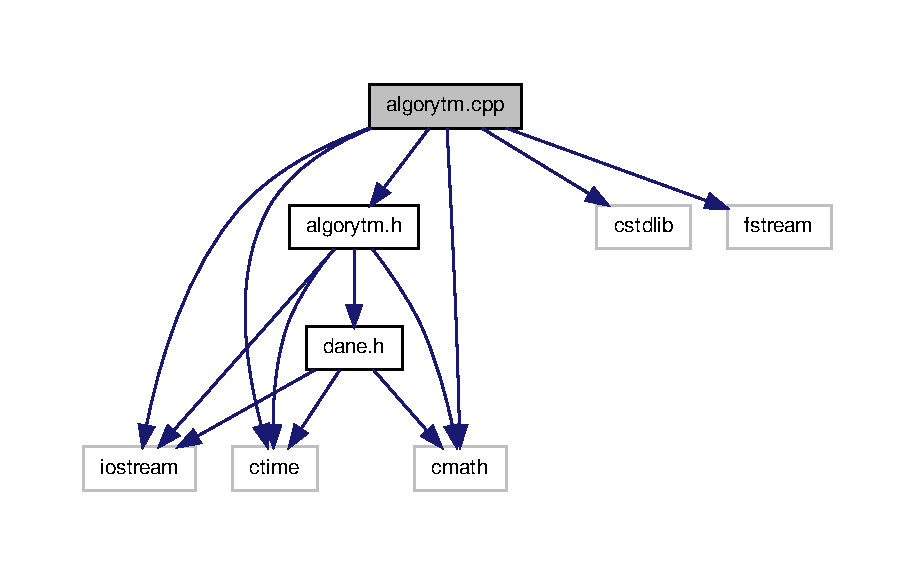
\includegraphics[width=350pt]{algorytm_8cpp__incl}
\end{center}
\end{figure}


\subsection{Detailed Description}
Plik zawiera definicje metod klasy algorytm oraz przeciazenie operatora przypisania. Zdefiniowane sa tutaj metody odpowiadajace za wczytanie pliku z danymi oraz pliku z danymi sprawdzajacymi. Ponadto zdefiniowana sa metody pobrania czasu, wykonania obliczen algorytmu, sprawdzajaca poprawnosc obliczen oraz test algorytmu. w tym miejsu również znajduja sie definicje operacji odwracania elementow tablicy, zamiany danych elementow, dodanie elementu do tablicy, dodanie dwoch tablic. Zdefiniowane sa tez pliki testowe dla operacji wczytywania danych do struktur danych min kolejki i stosu. 

Definition in file \hyperlink{algorytm_8cpp_source}{algorytm.\-cpp}.


\hypertarget{algorytm_8h}{\section{algorytm.\-h File Reference}
\label{algorytm_8h}\index{algorytm.\-h@{algorytm.\-h}}
}


Definicja klasy algorytm.  


{\ttfamily \#include $<$iostream$>$}\\*
{\ttfamily \#include $<$ctime$>$}\\*
{\ttfamily \#include $<$cmath$>$}\\*
{\ttfamily \#include \char`\"{}dane.\-h\char`\"{}}\\*
Include dependency graph for algorytm.\-h\-:\nopagebreak
\begin{figure}[H]
\begin{center}
\leavevmode
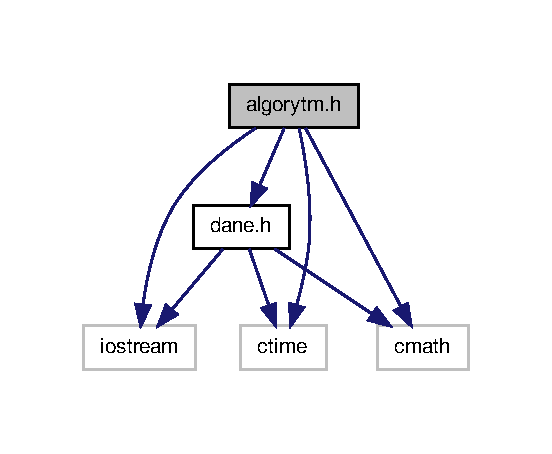
\includegraphics[width=265pt]{algorytm_8h__incl}
\end{center}
\end{figure}
This graph shows which files directly or indirectly include this file\-:\nopagebreak
\begin{figure}[H]
\begin{center}
\leavevmode
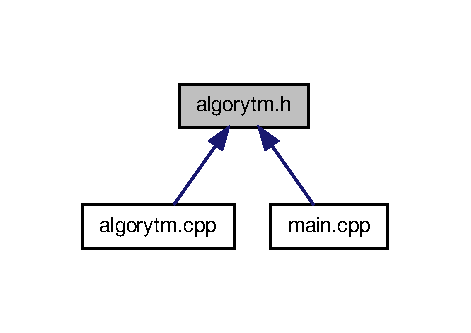
\includegraphics[width=226pt]{algorytm_8h__dep__incl}
\end{center}
\end{figure}
\subsection*{Classes}
\begin{DoxyCompactItemize}
\item 
class \hyperlink{classalgorytm}{algorytm}
\begin{DoxyCompactList}\small\item\em Modeluje pojecie algorytmu. \end{DoxyCompactList}\end{DoxyCompactItemize}


\subsection{Detailed Description}
Plik zawiera definicje klasy algorytm, ktora wykonuje niezbedne operacje na plikach tekstowych. 

Definition in file \hyperlink{algorytm_8h_source}{algorytm.\-h}.


\hypertarget{dane_8cpp}{\section{dane.\-cpp File Reference}
\label{dane_8cpp}\index{dane.\-cpp@{dane.\-cpp}}
}


Plik z definicjami metod dla klasy dane.  


{\ttfamily \#include $<$iostream$>$}\\*
{\ttfamily \#include $<$fstream$>$}\\*
{\ttfamily \#include $<$cmath$>$}\\*
{\ttfamily \#include $<$ctime$>$}\\*
{\ttfamily \#include \char`\"{}dane.\-h\char`\"{}}\\*
Include dependency graph for dane.\-cpp\-:\nopagebreak
\begin{figure}[H]
\begin{center}
\leavevmode
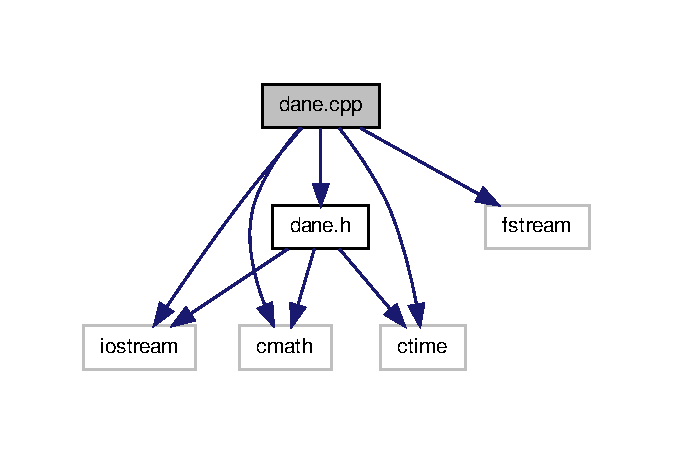
\includegraphics[width=323pt]{dane_8cpp__incl}
\end{center}
\end{figure}


\subsection{Detailed Description}
Plik zawiera definicje metod klasy dane tj. wyliczania wartosci odchylenia standardowego oraz zapisywania danych do pliku formatu csv. Ponadto zawiera definicje konstruktora parametrycznego w ktorym alokowana jest tablica do ktorej beda wpisywane czasy poszczegolnych powtorzen. 

Definition in file \hyperlink{dane_8cpp_source}{dane.\-cpp}.


\hypertarget{dane_8h}{\section{dane.\-h File Reference}
\label{dane_8h}\index{dane.\-h@{dane.\-h}}
}


Definicja klasy dane.  


{\ttfamily \#include $<$iostream$>$}\\*
{\ttfamily \#include $<$cmath$>$}\\*
{\ttfamily \#include $<$ctime$>$}\\*
Include dependency graph for dane.\-h\-:\nopagebreak
\begin{figure}[H]
\begin{center}
\leavevmode
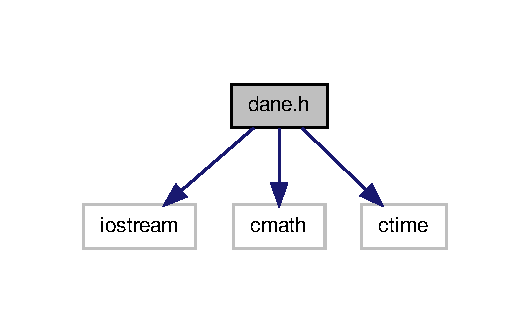
\includegraphics[width=254pt]{dane_8h__incl}
\end{center}
\end{figure}
This graph shows which files directly or indirectly include this file\-:\nopagebreak
\begin{figure}[H]
\begin{center}
\leavevmode
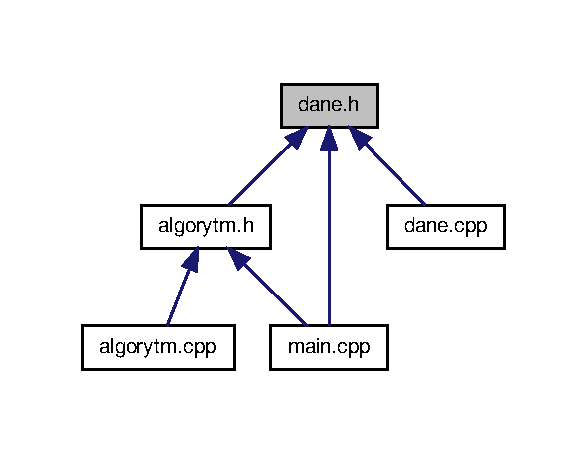
\includegraphics[width=282pt]{dane_8h__dep__incl}
\end{center}
\end{figure}
\subsection*{Classes}
\begin{DoxyCompactItemize}
\item 
class \hyperlink{classdane}{dane}
\begin{DoxyCompactList}\small\item\em Modeluje pojecie dane. \end{DoxyCompactList}\end{DoxyCompactItemize}


\subsection{Detailed Description}
Plik zawiera definicje klasy dane w ktorej znajduja sie informacje dotyczace wykonania algorytmu z powtorzeniami. 

Definition in file \hyperlink{dane_8h_source}{dane.\-h}.


\hypertarget{kolejka_8h}{\section{kolejka.\-h File Reference}
\label{kolejka_8h}\index{kolejka.\-h@{kolejka.\-h}}
}


Modeluje pojecie kolejki.  


{\ttfamily \#include $<$list$>$}\\*
{\ttfamily \#include $<$iostream$>$}\\*
Include dependency graph for kolejka.\-h\-:\nopagebreak
\begin{figure}[H]
\begin{center}
\leavevmode
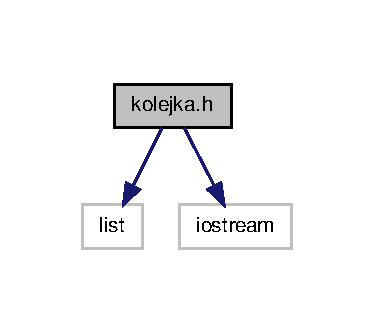
\includegraphics[width=180pt]{kolejka_8h__incl}
\end{center}
\end{figure}
This graph shows which files directly or indirectly include this file\-:\nopagebreak
\begin{figure}[H]
\begin{center}
\leavevmode
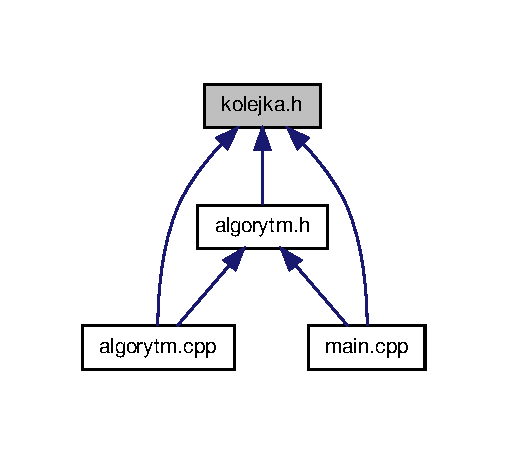
\includegraphics[width=244pt]{kolejka_8h__dep__incl}
\end{center}
\end{figure}
\subsection*{Classes}
\begin{DoxyCompactItemize}
\item 
class \hyperlink{classkolejkalist}{kolejkalist$<$ T\-Y\-P $>$}
\begin{DoxyCompactList}\small\item\em Definicja klasy kolejkalist. \end{DoxyCompactList}\item 
class \hyperlink{classkolejkatab}{kolejkatab$<$ T\-Y\-P $>$}
\begin{DoxyCompactList}\small\item\em Szablon klasy kolejkatab. \end{DoxyCompactList}\end{DoxyCompactItemize}


\subsection{Detailed Description}
W pliku znajduja sie defincije klas tworzacych strukture danych jaka jest kolejka. Pierwsza z klas opiera sie na szablonie listy z kontenera S\-T\-L druga zas opiera dzialanie na bazie tablicy alokowanej dynamicznie. 

Definition in file \hyperlink{kolejka_8h_source}{kolejka.\-h}.


\hypertarget{main_8cpp}{\section{main.\-cpp File Reference}
\label{main_8cpp}\index{main.\-cpp@{main.\-cpp}}
}


Funkcja main.  


{\ttfamily \#include $<$iostream$>$}\\*
{\ttfamily \#include $<$cstdlib$>$}\\*
{\ttfamily \#include \char`\"{}dane.\-h\char`\"{}}\\*
{\ttfamily \#include \char`\"{}algorytm.\-h\char`\"{}}\\*
{\ttfamily \#include \char`\"{}stos.\-h\char`\"{}}\\*
{\ttfamily \#include \char`\"{}kolejka.\-h\char`\"{}}\\*
Include dependency graph for main.\-cpp\-:\nopagebreak
\begin{figure}[H]
\begin{center}
\leavevmode
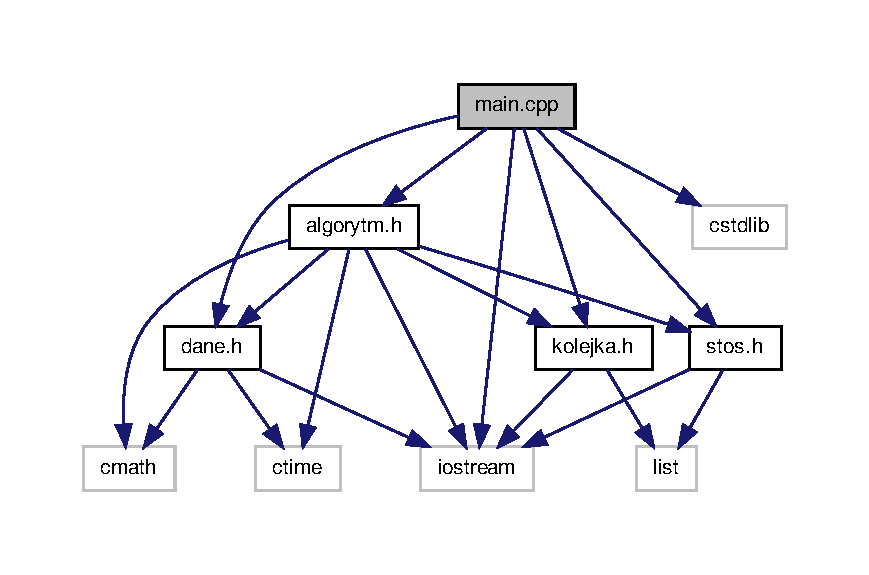
\includegraphics[width=350pt]{main_8cpp__incl}
\end{center}
\end{figure}
\subsection*{Functions}
\begin{DoxyCompactItemize}
\item 
int \hyperlink{main_8cpp_ae66f6b31b5ad750f1fe042a706a4e3d4}{main} ()
\end{DoxyCompactItemize}


\subsection{Detailed Description}
Plik zawiera glowna funkcje main w ktorej wywolywana jest metoda test obiektu algorytm. Ponadto w niej wczytywana jest do pola obiektu klasy algorytm liczba powtorzen wykonania algorytmu. Po wykonaniu wszystkich operacji funkcja zwraca zero.

\begin{DoxyReturn}{Returns}
Zwraca wartosc logiczna 0. 
\end{DoxyReturn}


Definition in file \hyperlink{main_8cpp_source}{main.\-cpp}.



\subsection{Function Documentation}
\hypertarget{main_8cpp_ae66f6b31b5ad750f1fe042a706a4e3d4}{\index{main.\-cpp@{main.\-cpp}!main@{main}}
\index{main@{main}!main.cpp@{main.\-cpp}}
\subsubsection[{main}]{\setlength{\rightskip}{0pt plus 5cm}int main (
\begin{DoxyParamCaption}
{}
\end{DoxyParamCaption}
)}}\label{main_8cpp_ae66f6b31b5ad750f1fe042a706a4e3d4}


Definition at line 22 of file main.\-cpp.



Here is the call graph for this function\-:
\nopagebreak
\begin{figure}[H]
\begin{center}
\leavevmode
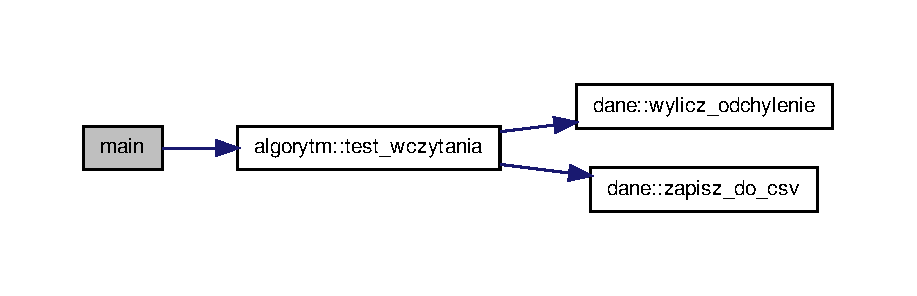
\includegraphics[width=350pt]{main_8cpp_ae66f6b31b5ad750f1fe042a706a4e3d4_cgraph}
\end{center}
\end{figure}



\hypertarget{stos_8h}{\section{stos.\-h File Reference}
\label{stos_8h}\index{stos.\-h@{stos.\-h}}
}


Modeluje pojecie stosu.  


{\ttfamily \#include $<$list$>$}\\*
{\ttfamily \#include $<$iostream$>$}\\*
Include dependency graph for stos.\-h\-:\nopagebreak
\begin{figure}[H]
\begin{center}
\leavevmode
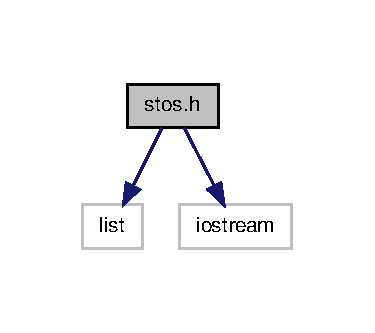
\includegraphics[width=180pt]{stos_8h__incl}
\end{center}
\end{figure}
This graph shows which files directly or indirectly include this file\-:\nopagebreak
\begin{figure}[H]
\begin{center}
\leavevmode
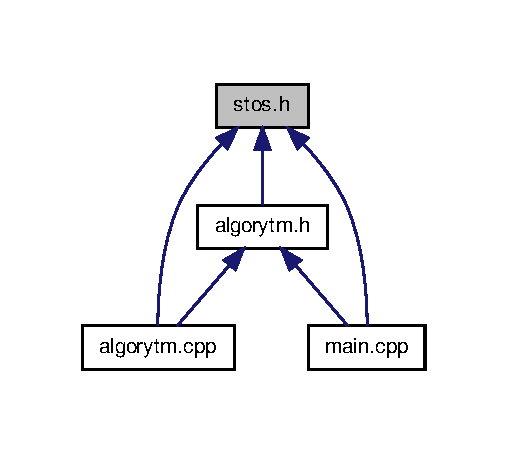
\includegraphics[width=244pt]{stos_8h__dep__incl}
\end{center}
\end{figure}
\subsection*{Classes}
\begin{DoxyCompactItemize}
\item 
class \hyperlink{classstoslist}{stoslist$<$ T\-Y\-P $>$}
\begin{DoxyCompactList}\small\item\em Definicja szablonu stoslist. \end{DoxyCompactList}\item 
class \hyperlink{classstostab}{stostab$<$ T\-Y\-P $>$}
\begin{DoxyCompactList}\small\item\em Definicja szablonu stostab. \end{DoxyCompactList}\end{DoxyCompactItemize}


\subsection{Detailed Description}
Plik definuje pojecie Stosu w oparciu o dwie klasy wykorzystujace inne metody implementacji struktury. Klasa stoslist wykorzystuje szablon S\-T\-L listy natomiast stostab implementuje tablice alokowana dynamicznie. 

Definition in file \hyperlink{stos_8h_source}{stos.\-h}.


\hypertarget{strona_8dox}{\section{strona.\-dox File Reference}
\label{strona_8dox}\index{strona.\-dox@{strona.\-dox}}
}

%--- End generated contents ---

% Index
\newpage
\phantomsection
\addcontentsline{toc}{part}{Index}
\printindex

\end{document}
